%%%%%%%%%%%%%%%%%%%%%%%%%%%%%%%%%%%%%%%%%
% Short Sectioned Assignment
% LaTeX Template
% Version 1.0 (5/5/12)
%
% This template has been downloaded from:
% http://www.LaTeXTemplates.com
%
% Original author:
% Frits Wenneker (http://www.howtotex.com)
%
% License:
% CC BY-NC-SA 3.0 (http://creativecommons.org/licenses/by-nc-sa/3.0/)
%
%%%%%%%%%%%%%%%%%%%%%%%%%%%%%%%%%%%%%%%%%

%----------------------------------------------------------------------------------------
%   PACKAGES AND OTHER DOCUMENT CONFIGURATIONS
%----------------------------------------------------------------------------------------

\documentclass[paper=a4, fontsize=11pt]{scrartcl} % A4 paper and 11pt font size

%\usepackage[T1]{fontenc} % Use 8-bit encoding that has 256 glyphs
%\usepackage{fourier} % Use the Adobe Utopia font for the document - comment this line to return to the LaTeX default
\usepackage[english]{babel} % English language/hyphenation
\usepackage{amsmath,amsfonts,amsthm,bm} % Math packages

\usepackage{sectsty} % Allows customizing section commands
\allsectionsfont{\centering \normalfont\scshape} % Make all sections centered, the default font and small caps
\usepackage{graphicx}
\usepackage{float}

\usepackage{listings}
\usepackage{color} %red, green, blue, yellow, cyan, magenta, black, white
\definecolor{mygreen}{RGB}{28,172,0} % color values Red, Green, Blue
\definecolor{mylilas}{RGB}{170,55,241}

\lstset{language=Matlab,%
    %basicstyle=\color{red},
    breaklines=true,%
    basicstyle=\small,
    morekeywords={matlab2tikz},
    keywordstyle=\color{black},%
    morekeywords=[2]{1}, keywordstyle=[2]{\color{black}},
    identifierstyle=\color{black},%
    stringstyle={\color{mylilas}},
    commentstyle={\tiny \color{mygreen}},%
    showstringspaces=false,%without this there will be a symbol in the places where there is a space
    numbers=left,%
    numberstyle={\tiny \color{black}},% size of the numbers
    numbersep=9pt, % this defines how far the numbers are from the text
    emph=[1]{for,function,end,if,while,break},emphstyle=[1]\color{blue}, %some words to emphasise
    xleftmargin=0.5in,
    xrightmargin=0.5in
    %emph=[2]{word1,word2}, emphstyle=[2]{style},    
}

\usepackage{fancyhdr} % Custom headers and footers
\pagestyle{fancyplain} % Makes all pages in the document conform to the custom headers and footers
\fancyhead{} % No page header - if you want one, create it in the same way as the footers below
\fancyfoot[L]{} % Empty left footer
\fancyfoot[C]{} % Empty center footer
\fancyfoot[R]{\thepage} % Page numbering for right footer
\renewcommand{\headrulewidth}{0pt} % Remove header underlines
\renewcommand{\footrulewidth}{0pt} % Remove footer underlines
\setlength{\headheight}{13.6pt} % Customize the height of the header

\numberwithin{equation}{section} % Number equations within sections (i.e. 1.1, 1.2, 2.1, 2.2 instead of 1, 2, 3, 4)
\numberwithin{figure}{section} % Number figures within sections (i.e. 1.1, 1.2, 2.1, 2.2 instead of 1, 2, 3, 4)
\numberwithin{table}{section} % Number tables within sections (i.e. 1.1, 1.2, 2.1, 2.2 instead of 1, 2, 3, 4)

\setlength\parindent{0pt} % Removes all indentation from paragraphs - comment this line for an assignment with lots of text
\setlength{\parskip}{1em}

%----------------------------------------------------------------------------------------
%   TITLE SECTION
%----------------------------------------------------------------------------------------

\newcommand{\horrule}[1]{\rule{\linewidth}{#1}} % Create horizontal rule command with 1 argument of height

\title{ 
\normalfont \normalsize 
\textsc{CSULB Math 697} \\ [25pt] % Your university, school and/or department name(s)
\horrule{0.5pt} \\[0.4cm] % Thin top horizontal rule
\huge Rapid Distortion Theory and Anisotropic Flow \\ % The assignment title
\horrule{2pt} \\[0.5cm] % Thick bottom horizontal rule
}

\author{Kristin Holmbeck} % Your name

\date{\normalsize\today} % Today's date or a custom date

\begin{document}

\maketitle % Print the title
\tableofcontents
\pagebreak

%----------------------------------------------------------------------------------------
%   PROBLEM 1
%----------------------------------------------------------------------------------------

\section{Introduction to Fluid Dynamics}

\subsection{Navier-Stokes}

The Navier-Stokes equations describe the motion of viscous fluid flow in which the derivations are simply a matter of applying Newton's second law to fluid conservation laws. For the simplest case, these equations can be reduced by assuming \textit{incompressibility} of the fluid, that is, the fluid density does not change. Such fluids are called Newtonian fluids, and include water, air, and alcohol -- all incompressible fluids. 
In this case of incompressible flow, we have as the Navier-Stokes equations:

\begin{align} 
\begin{split}
    \frac{D \bm{u}}{Dt} = 
    \bm{u_t} + \left( \bm{u} \cdot \nabla \bm{u} \right) &=
         \frac{\mu}{\rho_0} \Delta \bm{u} - \frac{1}{\rho_0} \nabla p + \Vec{F}_{ext}
\end{split}             
\end{align}

where $\mu$ is the dynamic viscosity, $\rho_0$ is the uniform fluid density, $p$ is the pressure,
and $\Vec{F}_{ext}$ represents external forces, such as gravity. The solution vector 
$\bm{u} = \begin{bmatrix} u_1 & u_2 & u_3 \end{bmatrix}^T$ is the three-dimensional flow velocity. 
The notation $\frac{D \Vec{u}}{Dt}$ is referred to as the \textit{substantial} or \textit{material} derivative.

\par

The condition for incompressible flow -- also known as a \textit{solenoidal} vector field -- comes from the constant density of the fluid in the continuity equation. The continuity equation states that the rate at which mass enters a system is equal to the rate at which mass leaves the system plus the accumulation of mass within the system \cite{pedlosky}. 

\begin{align}
    \frac{\partial \rho}{\partial t} + \nabla \cdot \left( \rho \bm{u} \right ) &= 0 \\
    0 + \left (\nabla \cdot \rho \right ) \bm{u} + \rho \left ( \nabla \cdot \bm{u} \right ) &= 0 \\
    \rho \left ( \nabla \cdot \bm{u} \right ) &= 0 \\
    \nabla \cdot \bm{u} &= 0 \qquad \text{the zero-divergence condition}
\end{align}

Thus, for incompressible flow, we have the zero-divergence condition derived above.

\iffalse
    source:  Wikipedia: incompressible flow

    \begin{align}
        m &= \int_V \rho dV \\
        \frac{\partial m}{\partial t} &= \int_S \bold{J} d\bold{S}  \qquad \text{by conservation of mass} \\
        m = \int_V \rho dV &= \int_S \bold{J} d\bold{S} \\
            &= - \int_V \left( \nabla \cdot \bold{J} \right) dV \qquad \text{by the divergence theorem} \\
        \text{therefore} \qquad \frac{\partial \rho}{\partial t} &= - \nabla \cdot \bold{J}
    \end{align}
\fi

\par

In the next few sections, we will explore background ideas behind turbulent flow to set up for derivation of the Rapid Distortion Theory (RDT) equations. 

%------------------------------------------------

\subsection{Turbulence}

Turbulent fluid flow is characterized by chaotic or rapid changes in pressure and velocity, which is also seemingly random and unpredictable \cite{pope}.
Turbulent flow is in contrast to laminar (or streamline) flow where fluid flows in parallel layers, 
with little to no disruptions or mixing between layers. An example of both types of flow can be seen in Figure 
\ref{fig:laminarvturbulent}.

Fluid turbulence can be characterized by the Reynolds number ($Re$), a dimensionless quantity defined by \cite{reynoldsnumber}: 

\begin{align}
    Re &= \frac{\rho u L}{\mu}  
\end{align}

where $u$ is the relative velocity of the fluid, $L$ is a characteristic linear dimension, and $\mu$ is the dynamic viscosity of the fluid. The critical Reynolds number, $Re_{crit}$, is the threshold where laminar flow ceases to exist (the flow becomes turbulent), and is different depending on the shape and friction coefficient of the boundary layer 
\cite{reynoldshistory}.

For turbulent flow, we typically decompose the flow field into its mean and fluctuating components:
\begin{align} 
    \bm{u} &= \langle \bm{u} \rangle + \Vec{f}
\end{align}
where it is assumed that the time-averaged mean of the fluctuating component $\Vec{f}$ is zero. This is representation is known as the Reynolds decomposition.

\begin{figure}[!b]
    \centering
    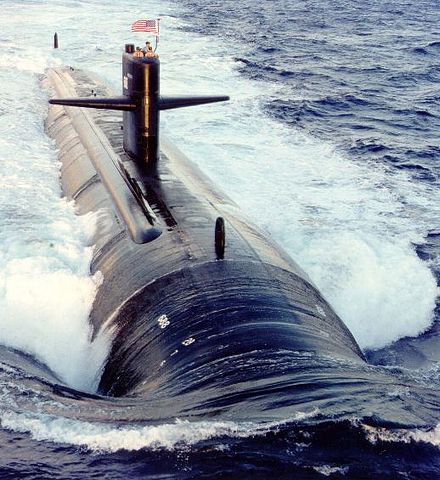
\includegraphics[width=2in]{laminar_v_turbulent.jpg}
    \caption{Laminar and turbulent water flow over the hull of a submarine. As the relative velocity of the water increases turbulence occurs.}
    \label{fig:laminarvturbulent}
\end{figure}

%------------------------------------------------

\subsection{Vorticity}

In both laminar and turbulent flows, we have rotational velocity of the fluid -- i.e. we have 
non-zero vorticity ($\bm{\omega}$). The vorticity can be obtained by taking the curl of the velocity

\begin{align}
    \bm{\omega} = \nabla \times \bm{u}
\end{align}

The purpose of including this section is for completeness. Vorticity is used in the derivation of the Rapid Distortion Theory equations, which we do not derive in this paper.
%------------------------------------------------

\subsection{Strain}

The deformation of a viscous fluid is called \textit{strain} -- the response of a system
to an applied force (\textit{stress}). There are generally three types of stress: tensional,
compression, and shear. For the purposes of this project, we will explore rapid shear stresses.

The rate of change of this deformation is represented in the strain rate tensor (the Jacobian of the velocity field):

\begin{align}
    \begin{bmatrix}
        \dfrac{\partial u_1}{\partial x_1} && \dfrac{\partial u_1}{\partial x_2} && \dfrac{\partial u_1}{\partial x_3} \\
        \\
        \dfrac{\partial u_2}{\partial x_1} && \dfrac{\partial u_2}{\partial x_2} && \dfrac{\partial u_2}{\partial x_3} \\
        \\
        \dfrac{\partial u_3}{\partial x_1} && \dfrac{\partial u_3}{\partial x_2} && \dfrac{\partial u_3}{\partial x_3} \\
    \end{bmatrix}
\end{align}


For simple shear stress in fluids (Figure \ref{fig:simpleshearstress}), we have the following:
\begin{align}
    \frac{\partial \langle u_1 \rangle}{\partial x_1} 
        &= \frac{\partial \langle u_2 \rangle}{\partial x_2}
        = \frac{\partial \langle u_3 \rangle}{\partial x_3}
        = 0 \\
    \frac{\partial \langle u_1 \rangle}{\partial x_2} &= \mathcal{S} \\
    \text{i.e. the shear rate tensor is:} \qquad
    &
    \begin{bmatrix}
        0 && \mathcal{S} && 0 \\
        0 && 0 && 0 \\
        0 && 0 && 0
    \end{bmatrix}\label{shearTensor}
\end{align}

The \textit{mean} strain rate tensor is defined as the average of the Jacobian matrix of the velocity field 
and the transpose of the Jacobian.

\begin{align}
    S^{ij} &= \frac{1}{2} \left (  \frac{\partial u_i}{\partial x_j} + \frac{\partial u_j}{\partial x_i} \right ) 
            = \frac{1}{2} \left (  \partial_j u_i + \partial_i u_j \right ) \\
    S      &= \frac{1}{2} \left ( \nabla \bm{u} + \nabla \bm{u}^T \right )
\end{align}

\begin{figure}
    \centering
    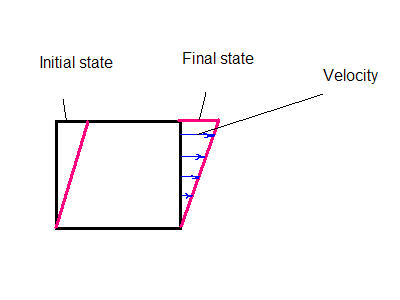
\includegraphics[width=4in]{../data/Simple_shear.PNG}
    \caption{Simple shear deformation}
    \label{fig:simpleshearstress}
\end{figure}

%------------------------------------------------

\subsection{Pressure}

The pressure rate-of-strain tensor comes from the Poisson equation for pressure. The Poisson
equation for $p^{'}$ is:

\begin{align}
    \frac{1}{\rho} \Delta p^{'} &= -2 \frac{ \partial \langle u_i \rangle }{\partial x_j}
            \frac{\partial f_j}{\partial x_i} - \frac{\partial^2}{\partial x_i \partial x_j}
            \left( 
                f_i f_j - \langle f_i f_j \rangle 
            \right ) \\
    p^{'} &= p^{(r)} + p^{(s)} + p^{(h)}
\end{align}

The three terms of $p^{'}$ represent the rapid, slow, and harmonic pressure contributions, respectively.


\begin{align}
    \frac{1}{\rho} \Delta p^{(r)} &= -2 \frac{ \partial \langle u_i \rangle }{\partial x_j}
            \frac{\partial f_j}{\partial x_i} \\
    \frac{1}{\rho} \Delta p^{(s)} &= - \frac{\partial^2}{\partial x_i \partial x_j}
            \left( 
                f_i f_j - \langle f_i f_j \rangle 
            \right ) \\
    \Delta p^{(h)} &= 0
\end{align}

%------------------------------------------------

\subsection{Visualizing Flow Field Data}

The fluid flow consists of a velocity cube for each direction ($x,y,z$).
\begin{align}
    \bm{u}(x,y,z,t=0) &= randn \sin (\pi z) + y \cos(\pi y) + \frac{1}{10}\sin(10 \pi x)
    \label{eq1}
\end{align}


% mini page prevents pagebreaks

\textsc{Matlab} code for plotting a flow field at a single time point (an example of which is in Figure \ref{fig:exflow}).
\begin{lstlisting}
function fh = plotField(X,Y,Z, u)

    if nargin == 1
        u = X;
        siz = size(u);
        [X,Y,Z] = meshgrid(1:siz(2), 1:siz(1), 1:siz(3));
    end

    fh = figure(gcf);

    xmin = min(X(:));
    xmax = max(X(:));
    ymax = max(Y(:));
    ymin = min(Y(:));
    zmin = min(Z(:));

    hs = slice(X,Y,Z,u,[xmin,(xmax+xmin)/2,xmax],[ymin, ymax],zmin);
    set(hs,'FaceColor','interp','EdgeColor','none')
    colormap jet
    xlabel x; ylabel y; zlabel z;

end
\end{lstlisting}


This code has been provided for future reference.

\begin{figure}
    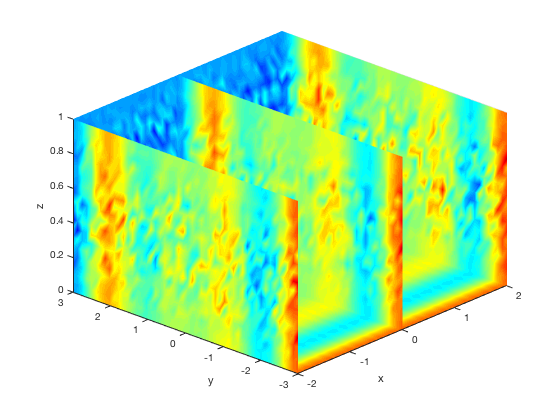
\includegraphics[width=\linewidth]{../data/fieldModesInit.png}
    \caption{Example flow field from eqn. \ref{eq1}}
    \label{fig:exflow}
\end{figure}

%---------------------------------------------------------------
%---------------------------------------------------------------
%---------------------------------------------------------------
%---------------------------------------------------------------

\pagebreak
\section{Rapid Distortion Theory}

Rapid Distortion Theory, or RDT, comes from the evolution of turbulence as the turbulence-to-mean-shear ratio becomes arbitrarily large. The derivation for the RDT equations can be found in \cite{pope}.

\iffalse
(change this to not copy word-for-word):
"Homogeneous turbulence can be subjected to time-dependent uniform mean velocity gradients, 
the magnitude of which can be characterized by":

\begin{align}
    \mathcal{S}(t) \equiv \left ( 2 \Bar{S_{ij}} \Bar{S_{ij}} \right )^{1/2} 
\end{align}

\fi

%------------------------------------------------
\subsection{Fourier Modes}

In place of vorticity, we can express the initial flow as the sum of Fourier modes. 
The transformation between the flow field in Fourier space and the real field is:

\begin{align}
    \bold{u}( \bold{x},t) &= \sum_{ \bm{\kappa}^o}  \bold{\hat{u}}(\bm{\kappa^o}, t) \cdot e^{i \bm{\kappa}(t) \cdot \bold{x}}
\end{align}

where $\bm{\kappa}(0) = \bm{\kappa^o} $ is the intial condition for the wavenumber vector, and denotes one of a set of potentially random wavenumbers.
Furthermore, the modes have associated conjugate pairs to ensure $\bold{u}(\bold{x},t)$ is real, e.g. for a single mode:

\begin{align}
    \bold{u}(\bold{x},t) &= \bold{\hat{u}}(\bm{\kappa}, t) \cdot  e^{i \bm{\kappa}(t) \cdot \bold{x}} + \bold{\hat{u}^*}(\bm{\kappa}, t) \cdot  e^{-i \bm{\kappa}(t) \cdot \bold{x}}
\end{align}


where
$
    %%\Vec{\kappa} = \kappa_0 \left ( \Vec{e_1}n_1 + \Vec{e_2}n_2 + \Vec{e_3}n_3 \right )  \qquad  n_i \in \mathbb{Z} \\
    e^{i \bm{\kappa}(t) \cdot \bold{x}} = e^{i \bm{\kappa} \cdot \bold{x}} = e^{i \kappa_1 x_1} e^{i \kappa_2 x_2} e^{i \kappa_3 x_3}
$, 
and $\bm{\hat{u}}^*$ denotes the complex conjugate of $\bm{\hat{u}}$.

A divergence-free field in the Fourier space follows as:
\begin{align}
    0 = \nabla \cdot \bold{u}( \bold{x},t) &= \nabla \cdot \left ( \sum_{ \bm{\kappa}^o}  \bold{\hat{u}}(\bm{\kappa^o}, t) e^{i \bm{\kappa}(t) \cdot \bold{x}} \right ) \\
    &= \sum_{ \bm{\kappa}^o}  \nabla \cdot \left ( \bold{\hat{u}}(\bm{\kappa^o}, t)  e^{i \bm{\kappa}(t) \cdot \bold{x}} \right )  \\
    &= \sum_{ \bm{\kappa}^o} \bold{\hat{u}}(\bm{\kappa^o}, t) \left (
        \frac{\partial}{\partial x_1} e^{i \bm{\kappa}(t) \cdot \bold{x}} + 
        \frac{\partial}{\partial x_2} e^{i \bm{\kappa}(t) \cdot \bold{x}} + 
        \frac{\partial}{\partial x_3} e^{i \bm{\kappa}(t) \cdot \bold{x}}
        \right ) \\
    &= \sum_{ \bm{\kappa}^o} \bold{\hat{u}}(\bm{\kappa^o}, t) 
        \left [ \kappa_1 \hat{u}_1 + \kappa_2 \hat{u}_2 + \kappa_3 \hat{u}_3
        \right ] 
        \cdot i e^{i \bm{\kappa}(t) \cdot \bold{x}}
\end{align}

For a single mode, this implies:

\begin{align} 
    0 = \kappa_1 \hat{u}_1 + \kappa_2 \hat{u}_2 + \kappa_3 \hat{u}_3 
      = \bm{\kappa}(t) \cdot \hat{\bold{u}}(t)
      \label{zdiv}
\end{align}


\subsubsection{Orthonormality} 
Given two wavenumber vectors $\bm{\kappa}_n, \bm{\kappa}_m$, the inner product is

\begin{align}
    \langle e^{i \bm{\kappa}_n \cdot \bm{x}}, e^{i \bm{\kappa}_m \cdot \bm{x}} \rangle_{\mathcal{L}}
    = \int_{\mathcal{L}} e^{i \bm{\kappa}_n \cdot \bm{x}}  e^{i \bm{\kappa}_m \cdot \bm{x}} dx
    = \left\{
    \begin{matrix} 
        0 \qquad m \neq n \\
        1 \qquad m = n
    \end{matrix} \right.
\end{align}

\iffalse
%------------------------------------------------
\subsubsection{Kolmogorov}

Eddies are localized regions of high-vorticity in a fluid (swirls). For high Reynolds numbers, Kolmogorov postulated that these eddies are essentially isotropic. This leads us to Kolmogorov energy spectrum:

\begin{align}
    \frac{1}{2} \langle \bold{u}_i \bold{u}_i \rangle
        &= \int_0^{\infty} E(k) dk \\
    E(k) &= C \varepsilon^\frac{2}{3} k^{-\frac{5}{3}}
\end{align}

for $\varepsilon$ the rate of energy dissapation, a universal constant $C$, and 
\fi
%------------------------------------------------


\subsubsection{Evolution of the Wavenumber}

\begin{align}
    \frac{d \kappa_l}{dt} &= -\kappa_j \frac{\partial \langle U_j \rangle}{\partial x_l}
                           = - \sum_j \kappa_j \frac{\partial \langle U_j \rangle}{\partial x_l}
\end{align}


which gives us the differential equations for the evolutions of the wavenumbers,
with $\bm{\kappa}(0) = \bm{\kappa}^o = \begin{bmatrix} \kappa_1^o && \kappa_2^o && \kappa_3^o \end{bmatrix}^T$.
\begin{align}
    \kappa_1(t) &= \kappa_1^o  \\
    \kappa_2(t) &= \kappa_2^o - \mathcal{S} \kappa_1^o t \\
    \kappa_3(t) &= \kappa_3^o
\end{align}

%------------------------------------------------
\subsection{RDT Equations}

The vectors in Fourier space evolve as:
\begin{align}
    \frac{d \hat{u}_j}{dt} = & -\hat{u}_k \frac{\partial \langle U_l \rangle}{ \partial x_k} \left ( \delta_{jl} 
       - 2 \frac{ \kappa_j \kappa_l }{|\kappa|^2} \right )  \qquad \text{sum over } k,l 
\end{align}

With $\delta_{jl}$ being the Kronecker delta. For simple shear flow, this reduces to:

\begin{align}
    \frac{d \hat{u}_j}{dt} &= \hat{u}_2 \frac{\partial \langle U_1 \rangle}{ \partial x_2} 
        \left ( 2 \frac{\kappa_j \kappa_1 }{|\kappa|^2} - \delta_{j,1}  \right )
\end{align}

Leading to the differential equations below. Again, this is for shear flow as defined in Equation \ref{shearTensor}.

\begin{align}
    \frac{d \hat{u_1}}{dt} &= \mathcal{S} \hat{u}_2
        \left (
            \frac{2 \left( \kappa_1^o \right )^2}{  | \bm{\kappa} |^2  } - 1 
        \right ) \\
    \frac{d \hat{u_2}}{dt} &= 2 \mathcal{S} \hat{u} _2
             \frac{ \kappa_1^o \kappa_2(t) }{  | \bm{\kappa} |^2  } 
        \\
    \frac{d \hat{u_3}}{dt} &= 2 \mathcal{S} \hat{u}_2 
             \frac{ \kappa_1^o \kappa_3^o }{  | \bm{\kappa} |^2  } 
\end{align}



%------------------------------------------------
\subsubsection{Solenoidal Condition for RDT}\label{rdt_zero_div}
For a sanity check, we will explore the solenoidal field condition for the RDT equations in the Fourier space.
\begin{align}
    0 &= \nabla \cdot \bm{u} \\
   0 &= \kappa_1 \hat{u}_1 + \kappa_2 \hat{u}_2 + \kappa_3 \hat{u}_3
\end{align}

For a single mode, from equation \ref{zdiv}. Taking the time derivative, we can explore constraints on the wavevector.

\begin{align}
    0 &= \frac{d}{dt} \left( \nabla \cdot \bm{u} \right ) \\
    0 &= \frac{d}{dt} \left( \kappa_1 \hat{u}_1 + \kappa_2 \hat{u}_2 + \kappa_3 \hat{u}_3 \right ) \\
    0 &= \kappa_1^o \frac{d\hat{u}_1}{dt} + 
        \kappa_2(t) \frac{d\hat{u}_2}{dt} + 
        \kappa_3^o \frac{d\hat{u}_3}{dt} + \dot{\kappa_2}(t) \hat{u}_1 
    \\
    0 &= \kappa_1^o \mathcal{S} \hat{u}_2 \left ( \frac{2 \left( \kappa_1^o \right )^2}{  | \bm{\kappa} |^2  } - 1 \right )
        + \kappa_2(t) 2 \mathcal{S} \hat{u} _2
             \frac{ \kappa_1^o \kappa_2(t) }{  | \bm{\kappa} |^2  } \\
    & \quad  + \kappa_3^o 2 \mathcal{S} \hat{u} _2
             \frac{ \kappa_1^o \kappa_3^o }{  | \bm{\kappa} |^2  } 
        - \mathcal{S} \kappa_1^o \hat{u_2} 
    \\
    0 &= \dfrac{\mathcal{S} \kappa_1^o \hat{u}_2}{| \bm{\kappa} |^2  } \left ( 
        2 \left( \kappa_1^o \right )^2 - | \bm{\kappa} |^2
        + 2 \left( \kappa_2(t) \right )^2 + \left( \kappa_3^o \right )^2 
        - | \bm{\kappa} |^2  \right ) 
    \\
    0 &= \dfrac{\mathcal{S} \kappa_1^o \hat{u}_2}{| \bm{\kappa} |^2  } \left ( 
        2 \left( \kappa_1^o \right )^2 - 2 | \bm{\kappa} |^2
        + 2 \left( \kappa_2(t) \right )^2 + \left( \kappa_3^o \right )^2 
        \right ) 
    \\
    0 &= \dfrac{\mathcal{S} \kappa_1^o \hat{u}_2}{| \bm{\kappa} |^2  } \left ( 
        2 | \bm{\kappa} |^2  - 2 | \bm{\kappa} |^2
        - 2 \left( \kappa_3^o \right )^2  + \left( \kappa_3^o \right )^2 
        \right ) 
    \\
    0 &= \dfrac{\mathcal{S} \kappa_1^o \hat{u}_2}{| \bm{\kappa} |^2  } \left ( 
        -  \left( \kappa_3^o \right )^2 
        \right ) 
    \\
    0 &= \dfrac{\mathcal{S} \hat{u}_2}{| \bm{\kappa} |^2  } \kappa_1^o 
        \left( \kappa_3^o \right )^2 
    \\
    \implies 0 &= \kappa_1^o  \left( \kappa_3^o \right )^2 
\end{align}

\iffalse
%------------------------------------------------

\paragraph{Heading on level 4 (paragraph)}


Aenean commodo ligula eget dolor. Aenean massa. Cum sociis natoque penatibus et magnis dis parturient montes, nascetur ridiculus mus. Donec quam felis, ultricies nec, pellentesque eu, pretium quis, sem.
\fi

%------------------------------------------------
\subsection{Simulations}

In this section, we present the results of a few simulations of RDT using 4th-order Runge-Kutta as the differential equation solver. Persistent values between runs are outlined in Table \ref{simparams} below.

\renewcommand{\arraystretch}{2}
\begin{center}
\begin{tabular}{ | p{4cm} | c  |}

    \hline
    RK4 step size $h$       &   0.05 \\ \hline
    time  vector &  0:0.01:1 \\ \hline
    grid size $n$ (number of points in each dimension) &   10 \\ \hline
    units for each dimension of cube & $\dfrac{2\pi}{n} [-1,1] $ \\ \hline
    wavevector $\bm{\kappa}$ & $[0.107, 0.144, 1.215 ]^T$ \\ \hline
    Shear force $\mathcal{S}$ & 100 \\ \hline
    initial condition $u(0)$ & random, seeded \\ \hline
    initial condition $v(0)$ & random, seeded \\ \hline
    initial condition $w(0)$ & 0 \\ \hline
\end{tabular}
\captionof{table}{Simulation Parameters} \label{simparams}
\end{center}

Throughout the following simulations, we vary the single-mode wavevector, $\bm{\kappa}$, to explore the evolution of the fluid velocity. The purpose of this is to reconcile the outcome from Section \ref{rdt_zero_div}, which will be explored further beyond the timeline of this course. 

\par
The following figures show the $x-, y-,$ and $z-$velocity components of the fluid flow, respectively, for the time point specified in the figure caption. The color axis is fixed for each velocity field for the duration of a simulation. Different points in time are presented to the reader to get a sense of the velocity profile, not to compare each simulation from frame-to-frame.

\subsubsection{Simulation 1: $\kappa_1 = 0$}
In this simulation, $\bm{\kappa} = [0, 0.144, 1.215 ]^T$.

    \setkeys{Gin}{width=7.5in, height=3in}
    \begin{figure}[h!]
        \centering
        \makebox[\textwidth]{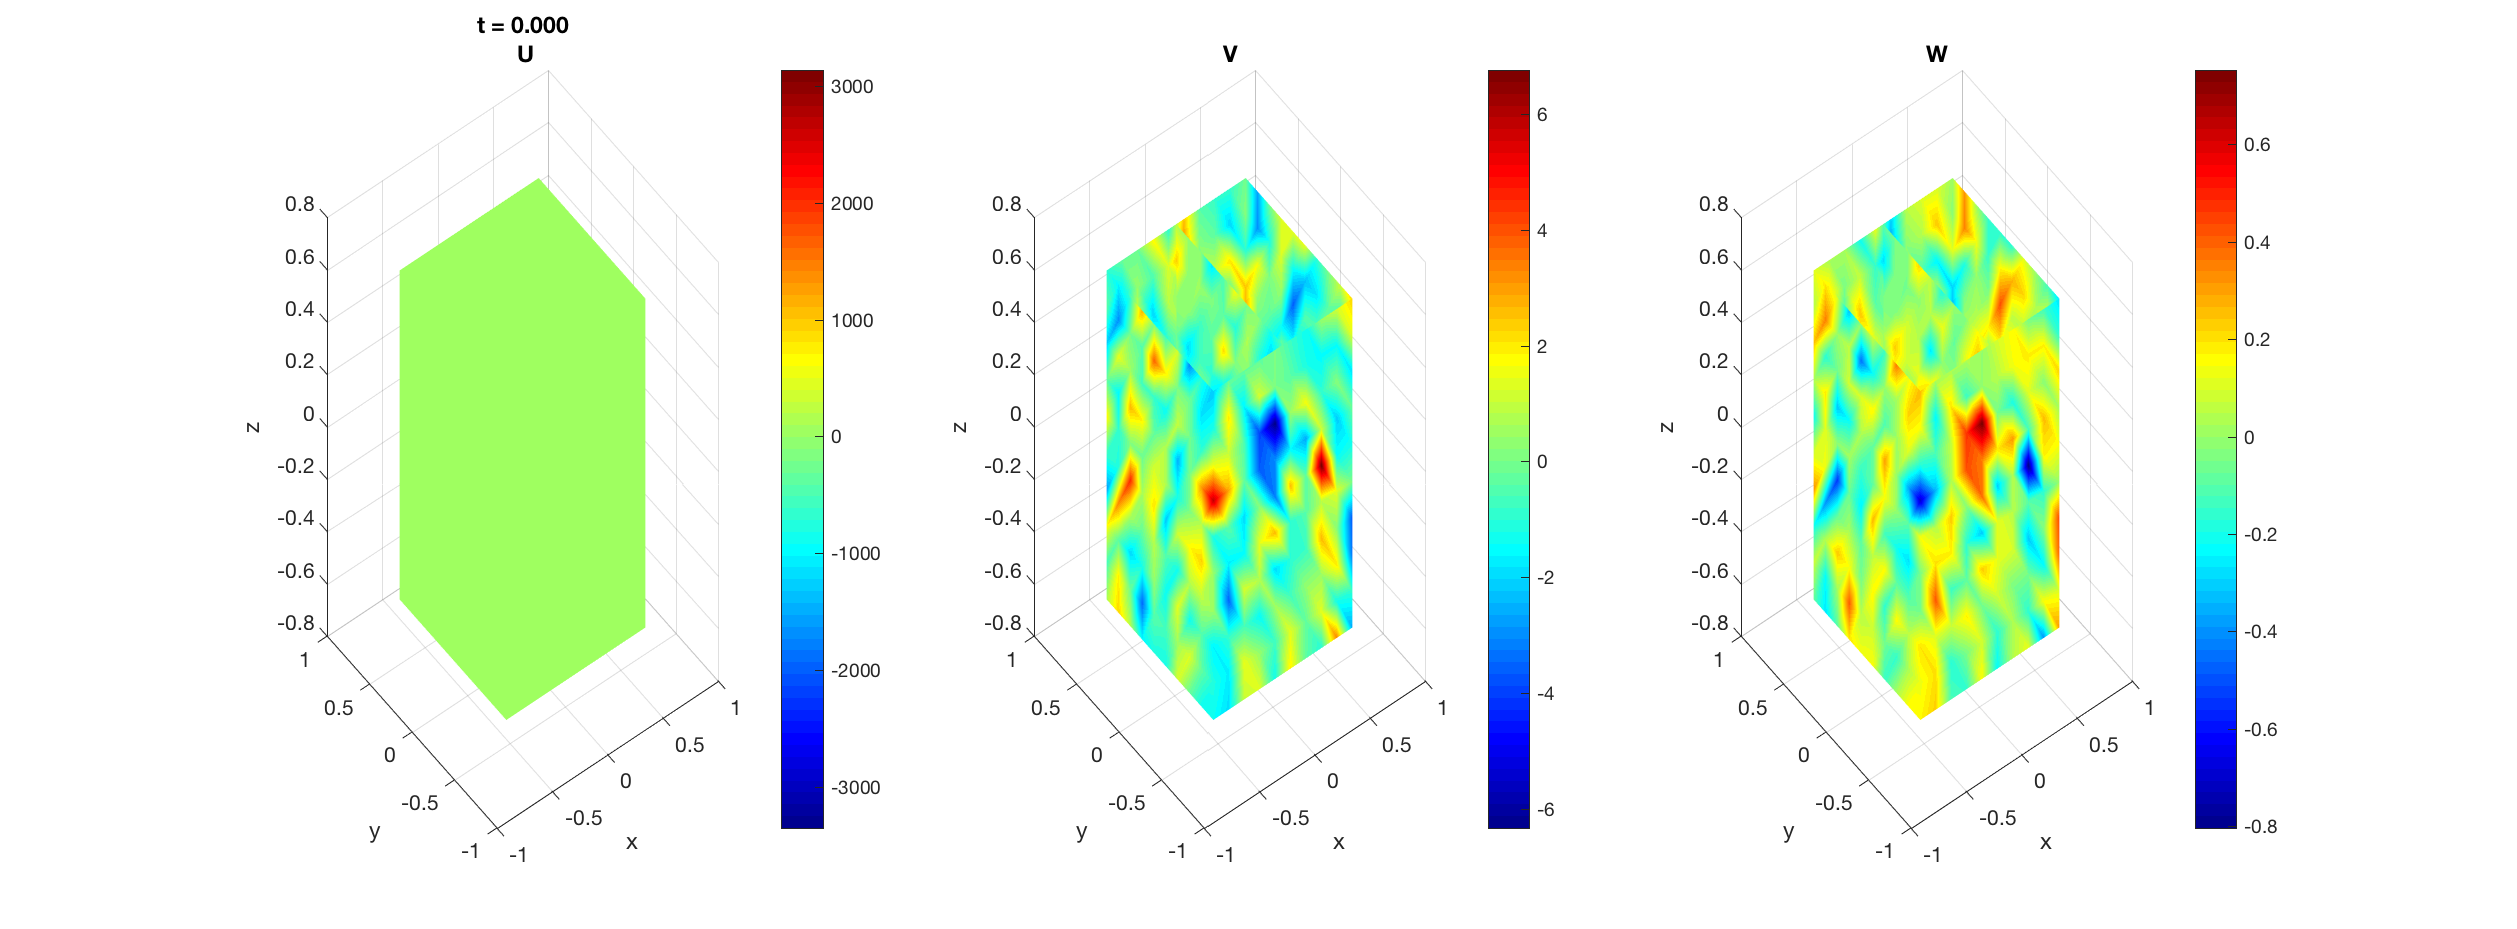
\includegraphics{../data/finalRuns/run1_frame1.png}}
        \caption{t = 0}
        \label{fig:frame1_1}
    \end{figure}
    \begin{figure}[h!]
        \makebox[\textwidth]{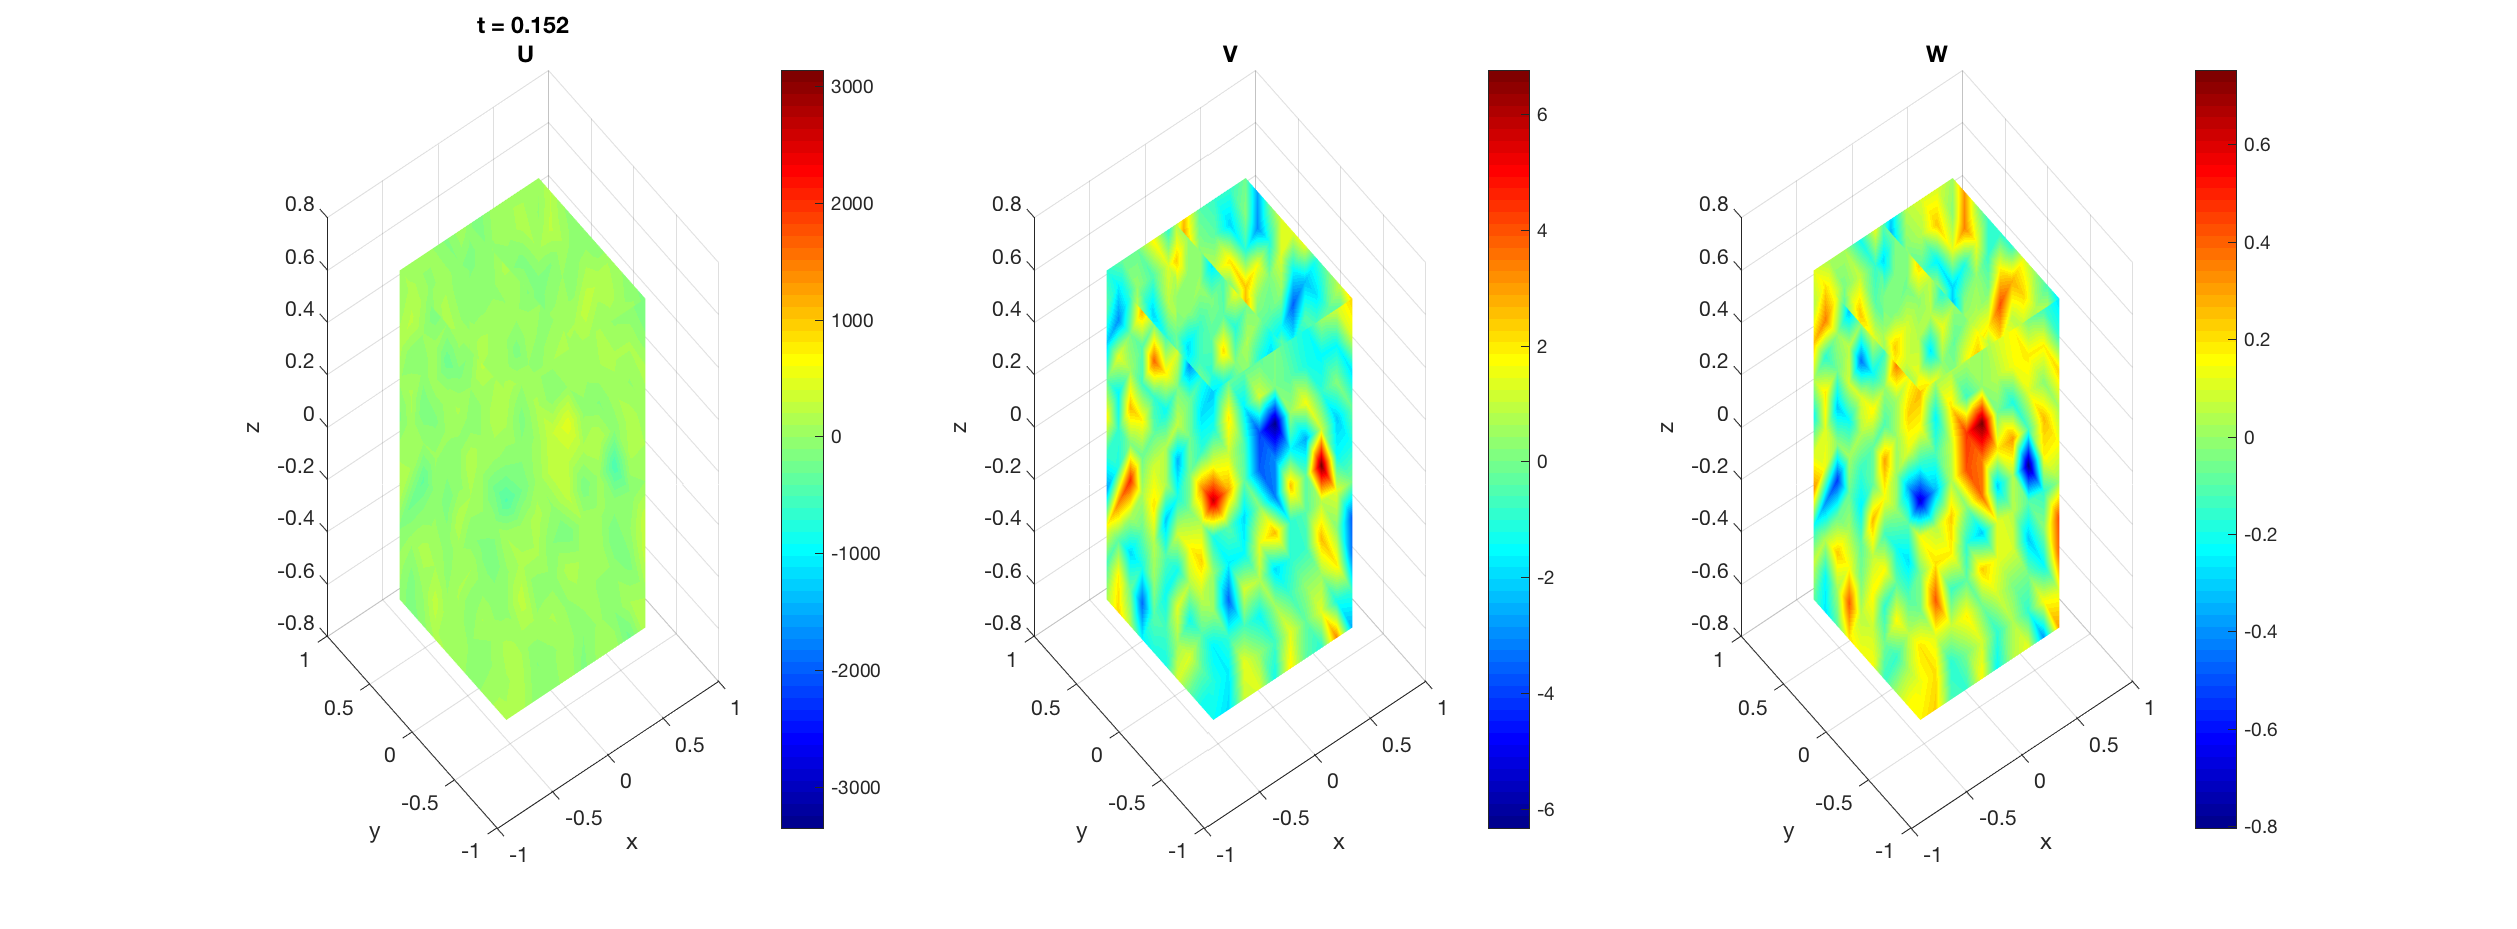
\includegraphics{../data/finalRuns/run1_frame16.png}}
        \caption{t = 0.152}
        \label{fig:frame1_16}
    \end{figure}
    \begin{figure}[H]
        \makebox[\textwidth]{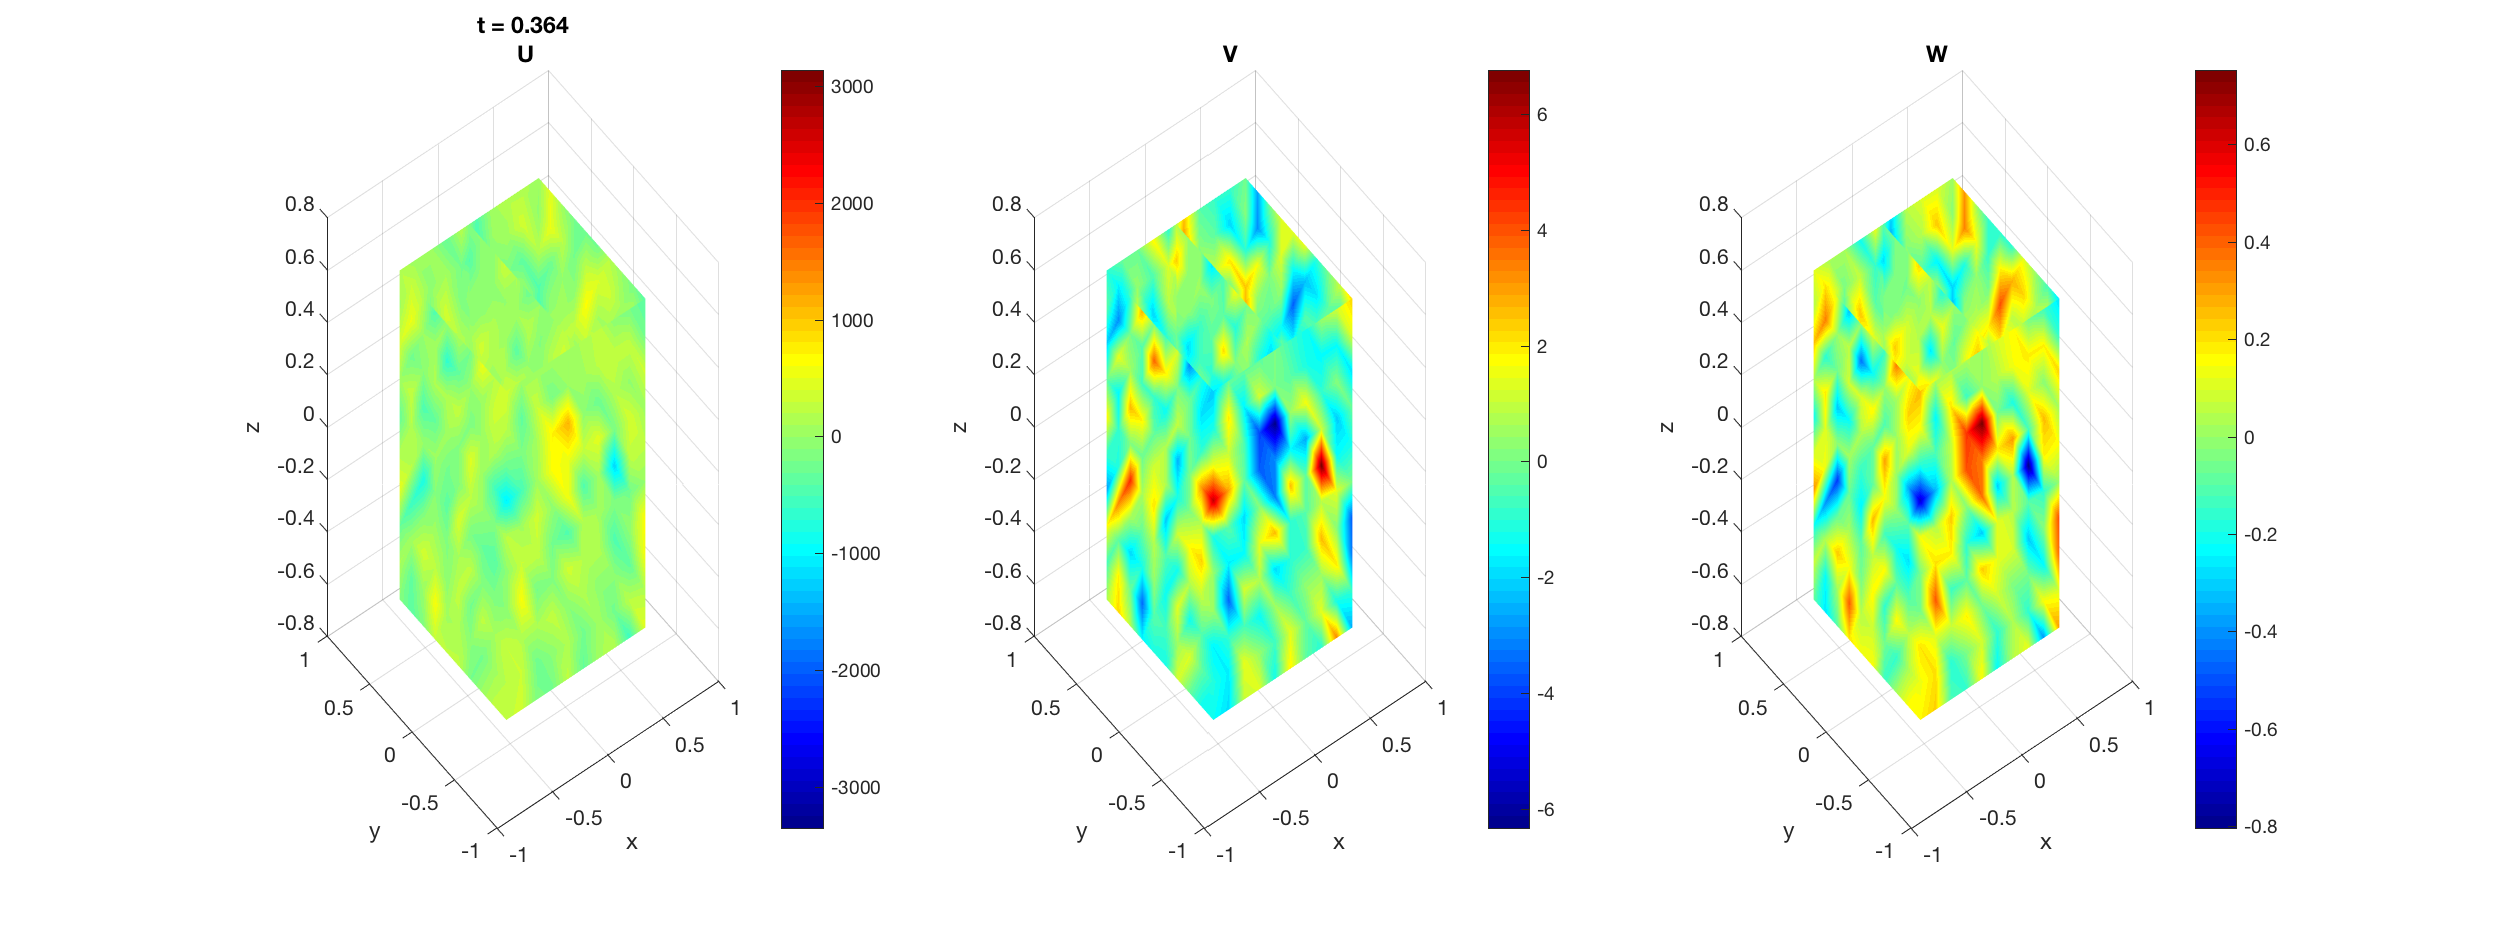
\includegraphics{../data/finalRuns/run1_frame37.png}}
        \caption{t = 0.364}
        \label{fig:frame1_37}
    \end{figure}
    \begin{figure}[h!]
        \makebox[\textwidth]{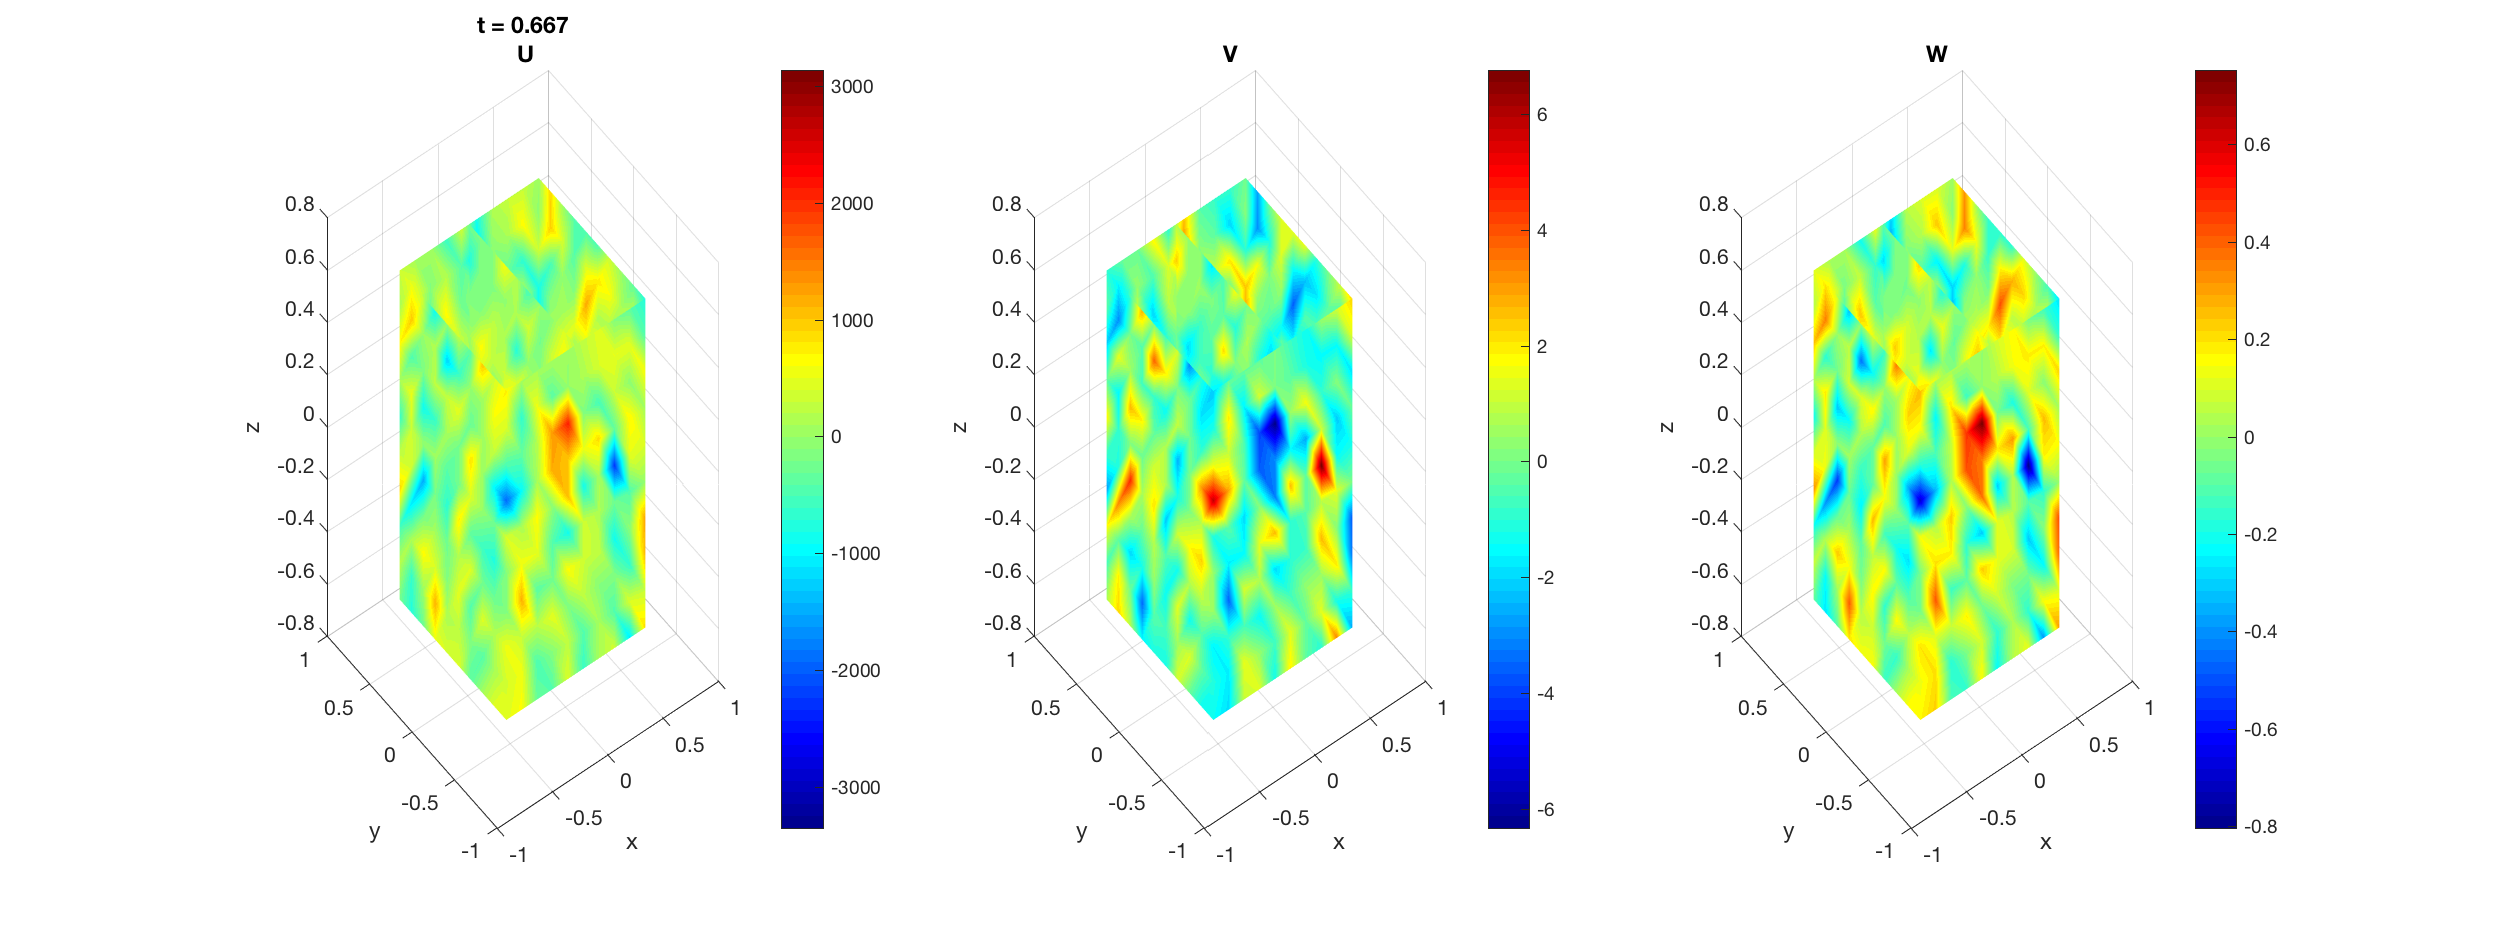
\includegraphics{../data/finalRuns/run1_frame67.png}}
        \caption{t = 0.667}
        \label{fig:frame1_67}
    \end{figure}
    \begin{figure}[h!]
        \makebox[\textwidth]{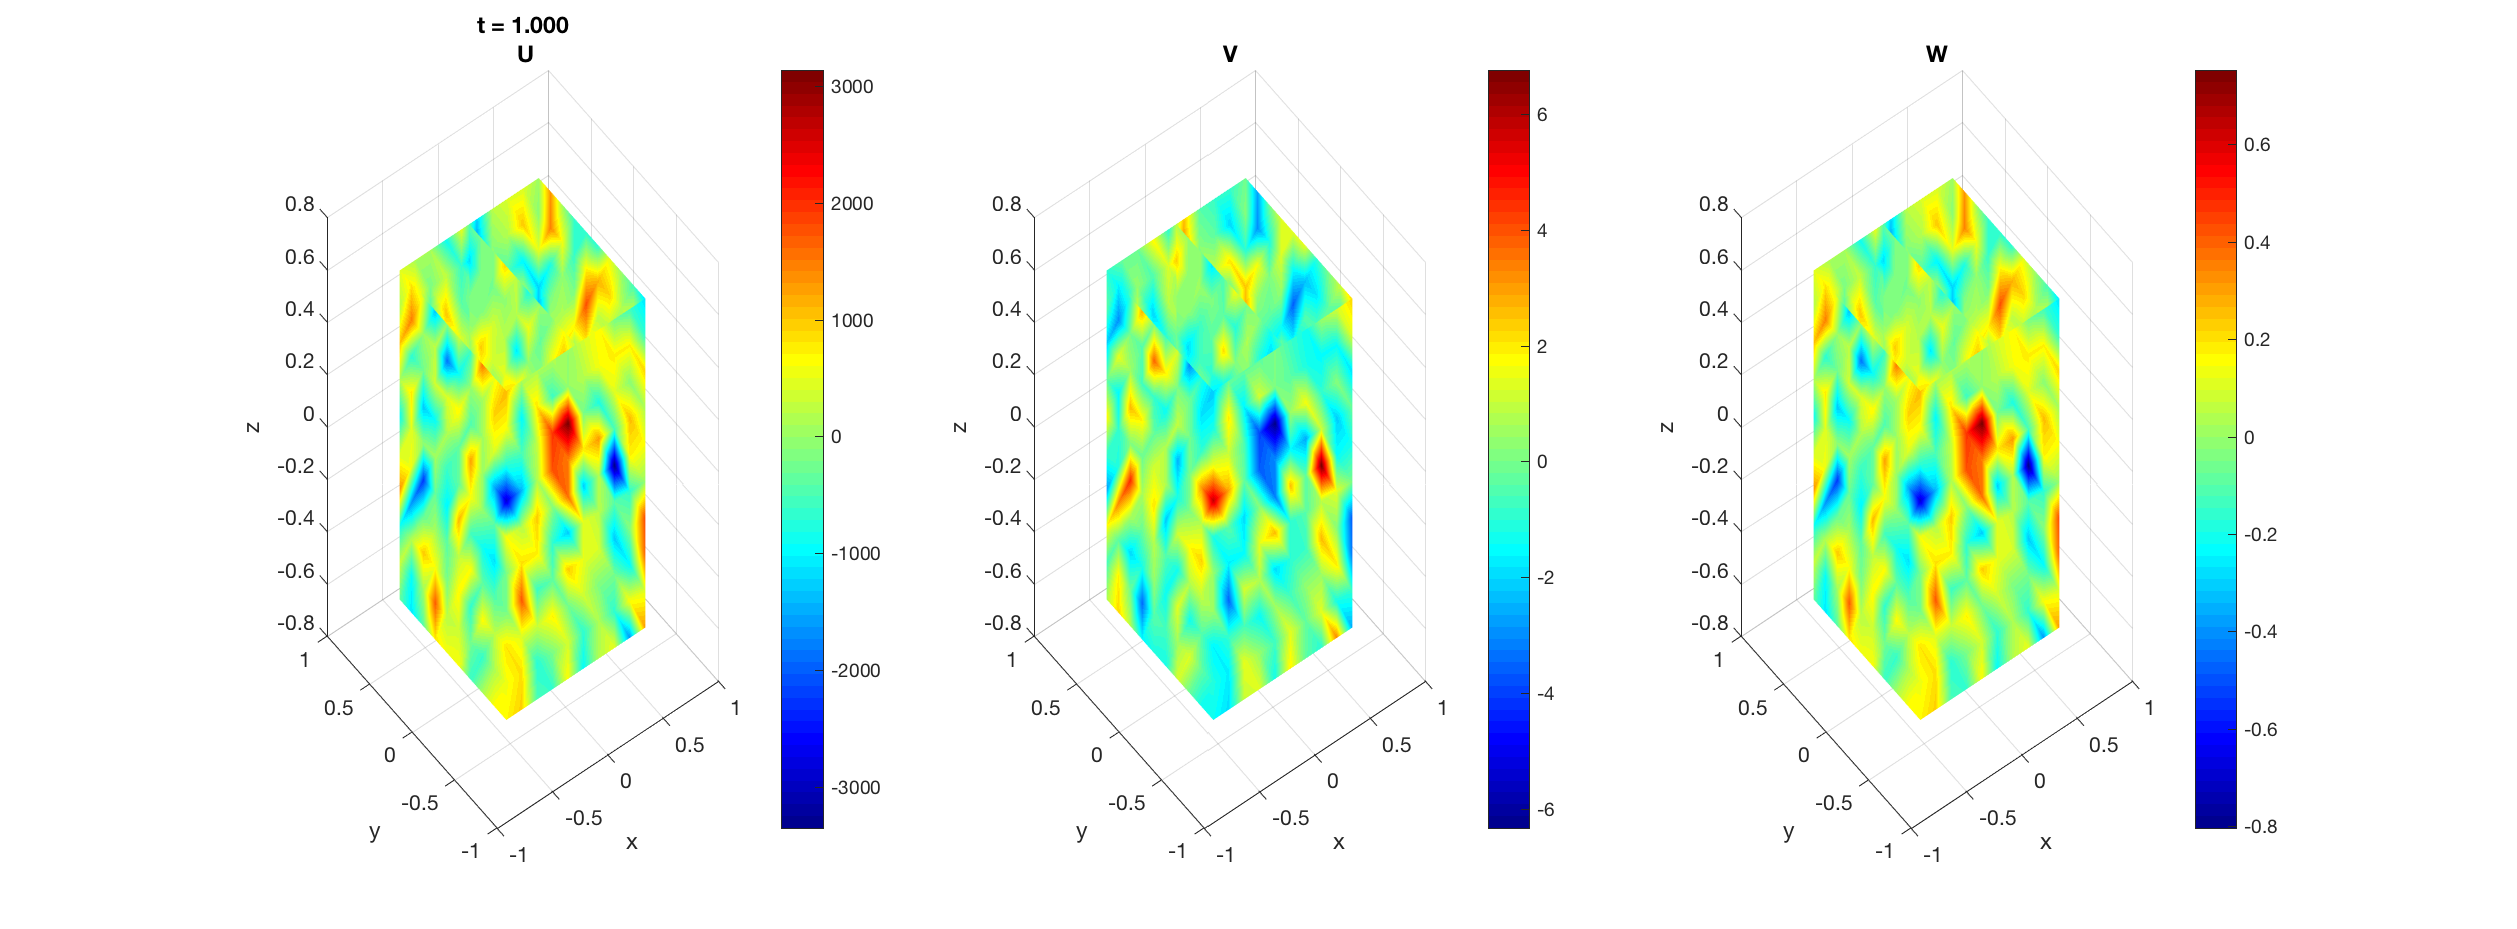
\includegraphics{../data/finalRuns/run1_frame100.png}}
        \caption{t = 1.0}
        \label{fig:frame1_100}
    \end{figure}

\subsubsection{Simulation 2: $\kappa_3 = 0$}
In this simulation, $\bm{\kappa} = [0.107, 0.144, 0 ]^T$.

    \begin{figure}[H]
        \centering
        \makebox[\textwidth]{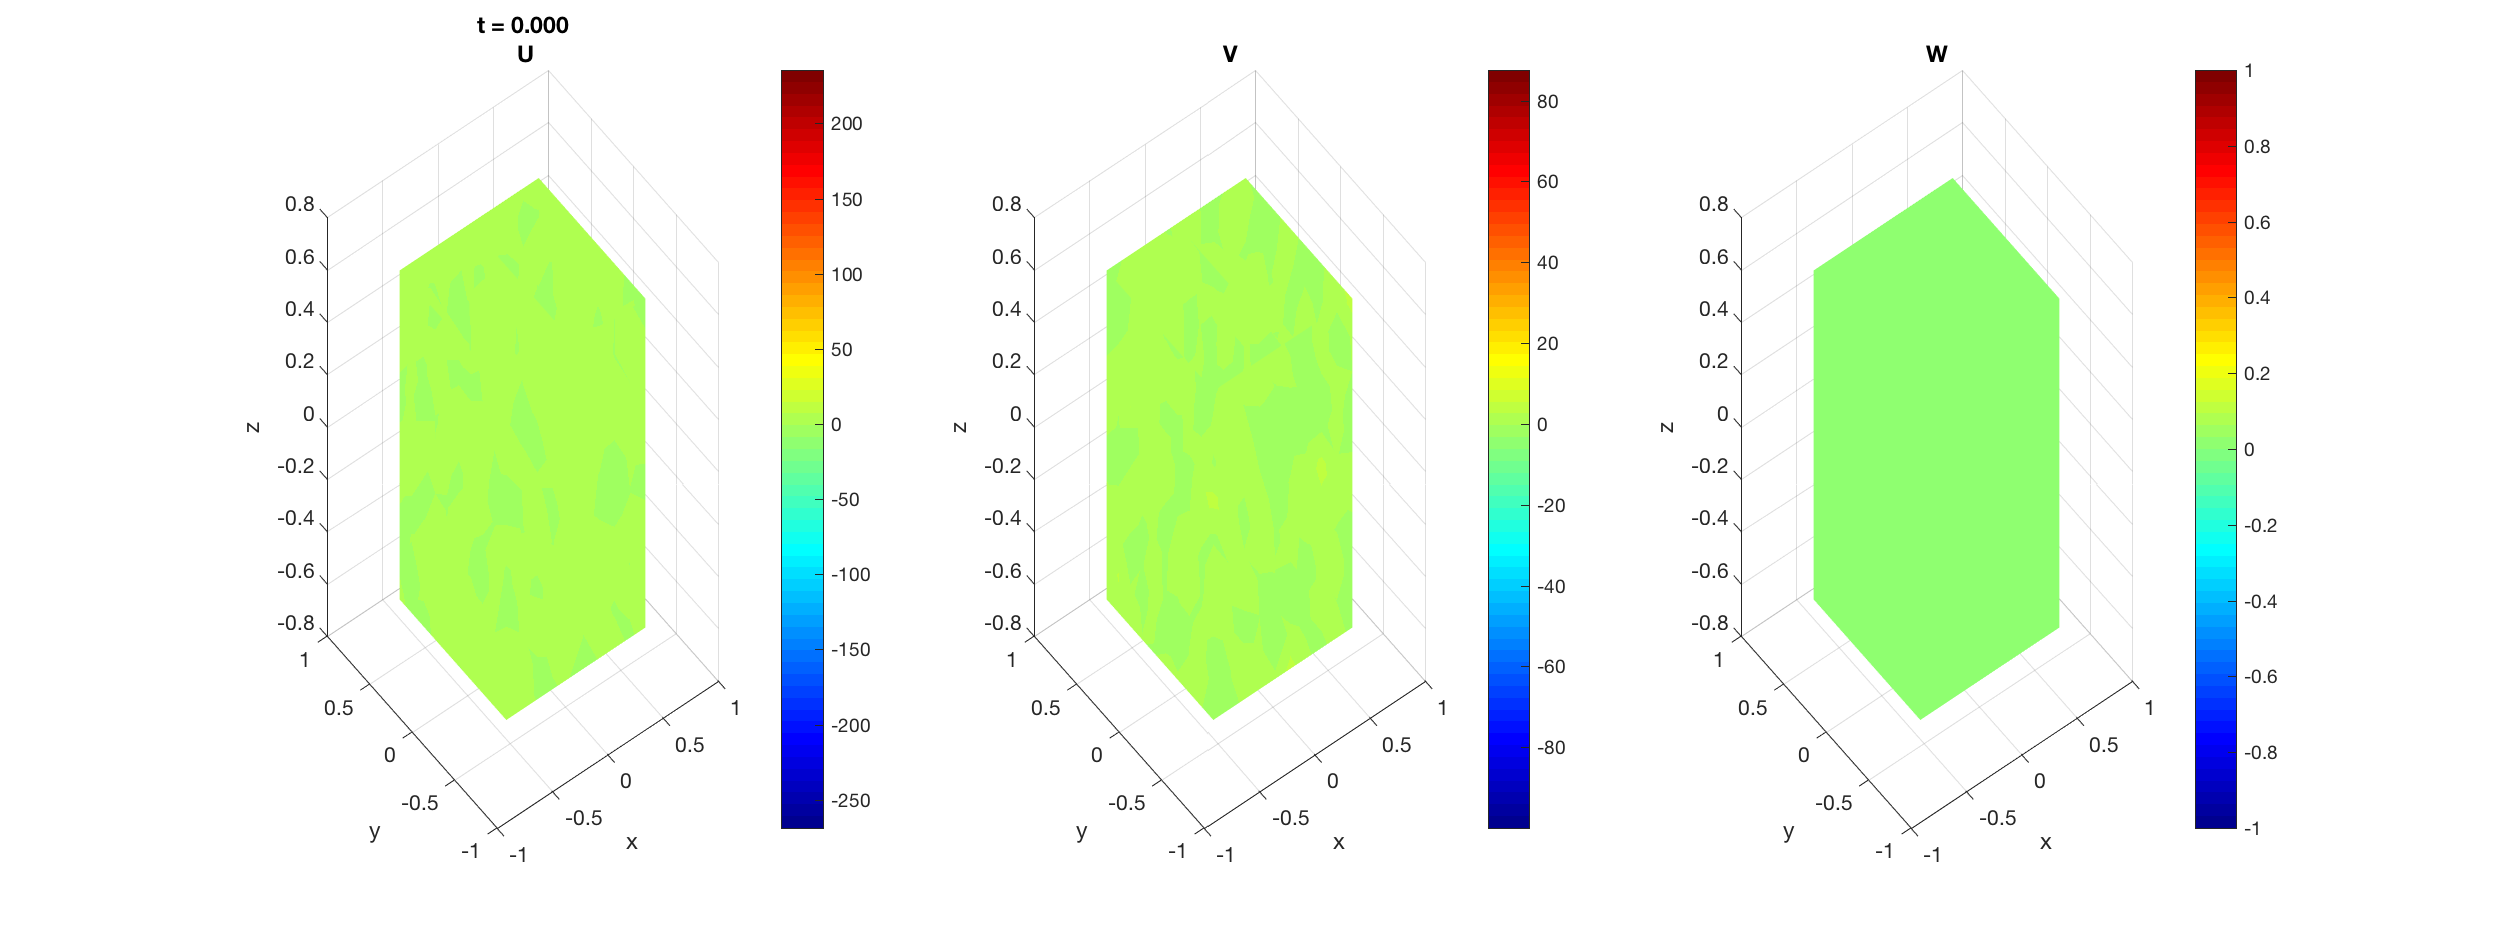
\includegraphics{../data/finalRuns/run2_frame1.png}}
        \caption{t = 0}
        \label{fig:frame2_1}
    \end{figure}
    \begin{figure}[H]
        \makebox[\textwidth]{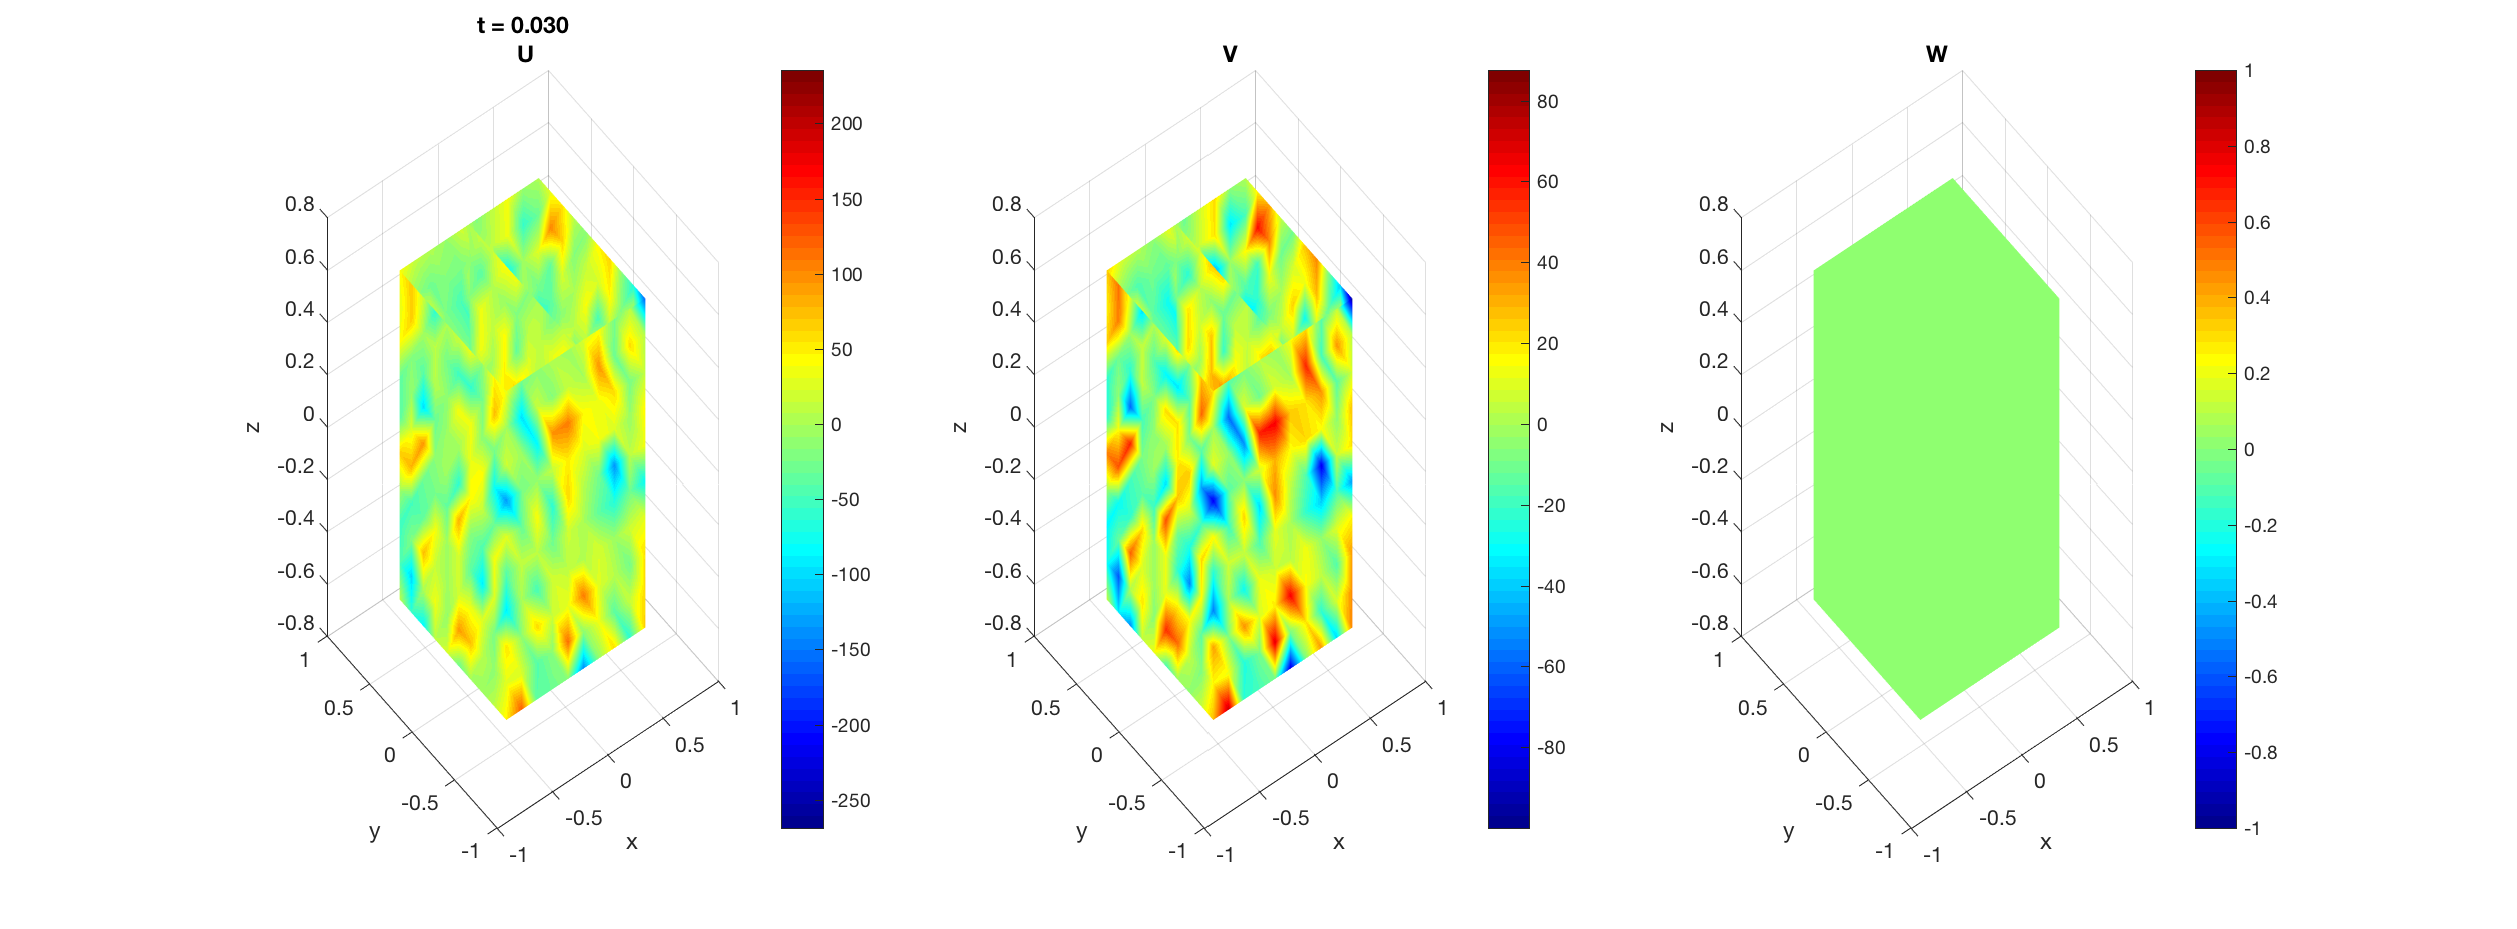
\includegraphics{../data/finalRuns/run2_frame4.png}}
        \caption{t = 0.030}
        \label{fig:frame2_4}
    \end{figure}
    \begin{figure}[H]
        \makebox[\textwidth]{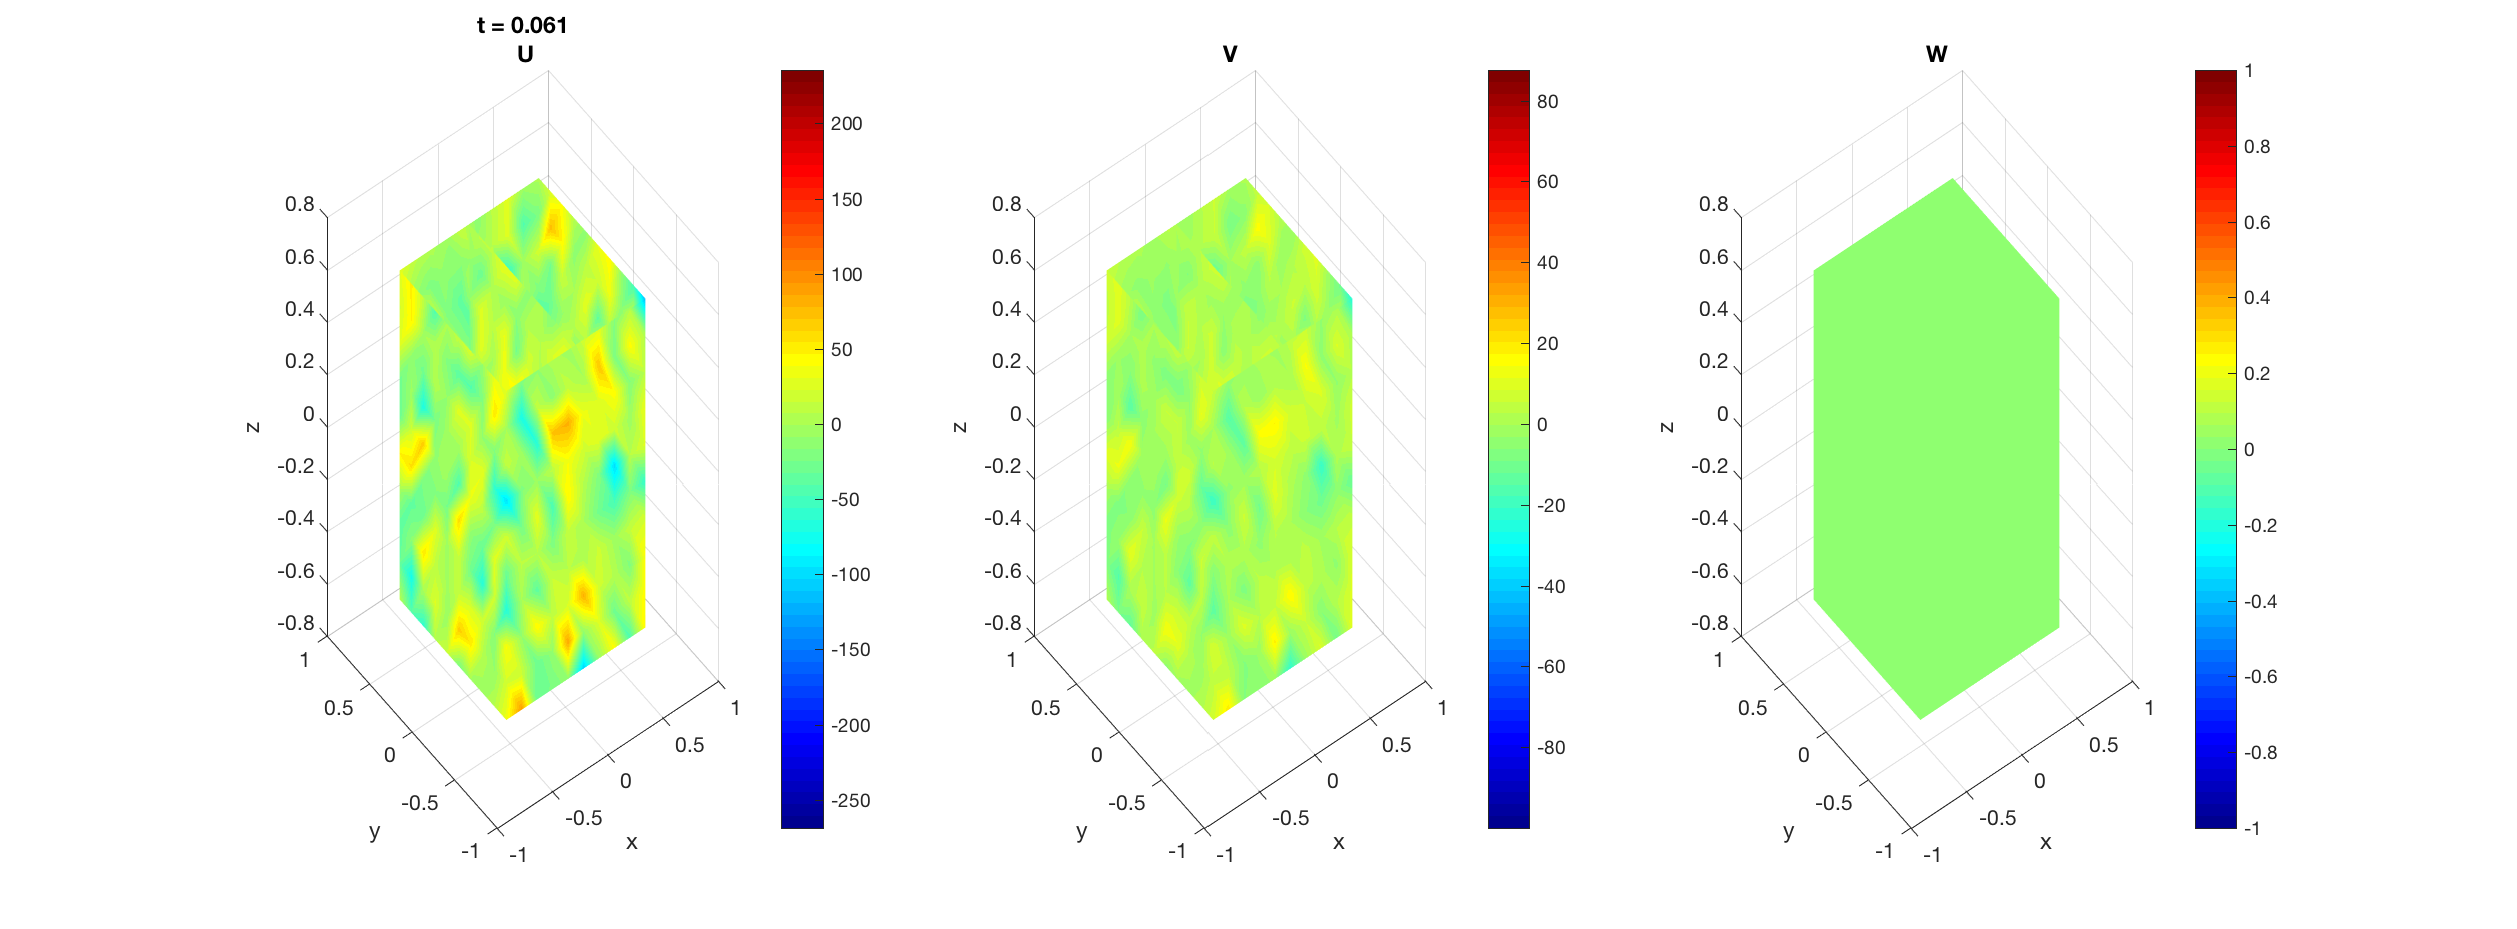
\includegraphics{../data/finalRuns/run2_frame7.png}}
        \caption{t = 0.061}
        \label{fig:frame2_7}
    \end{figure}
    \begin{figure}[H]
        \makebox[\textwidth]{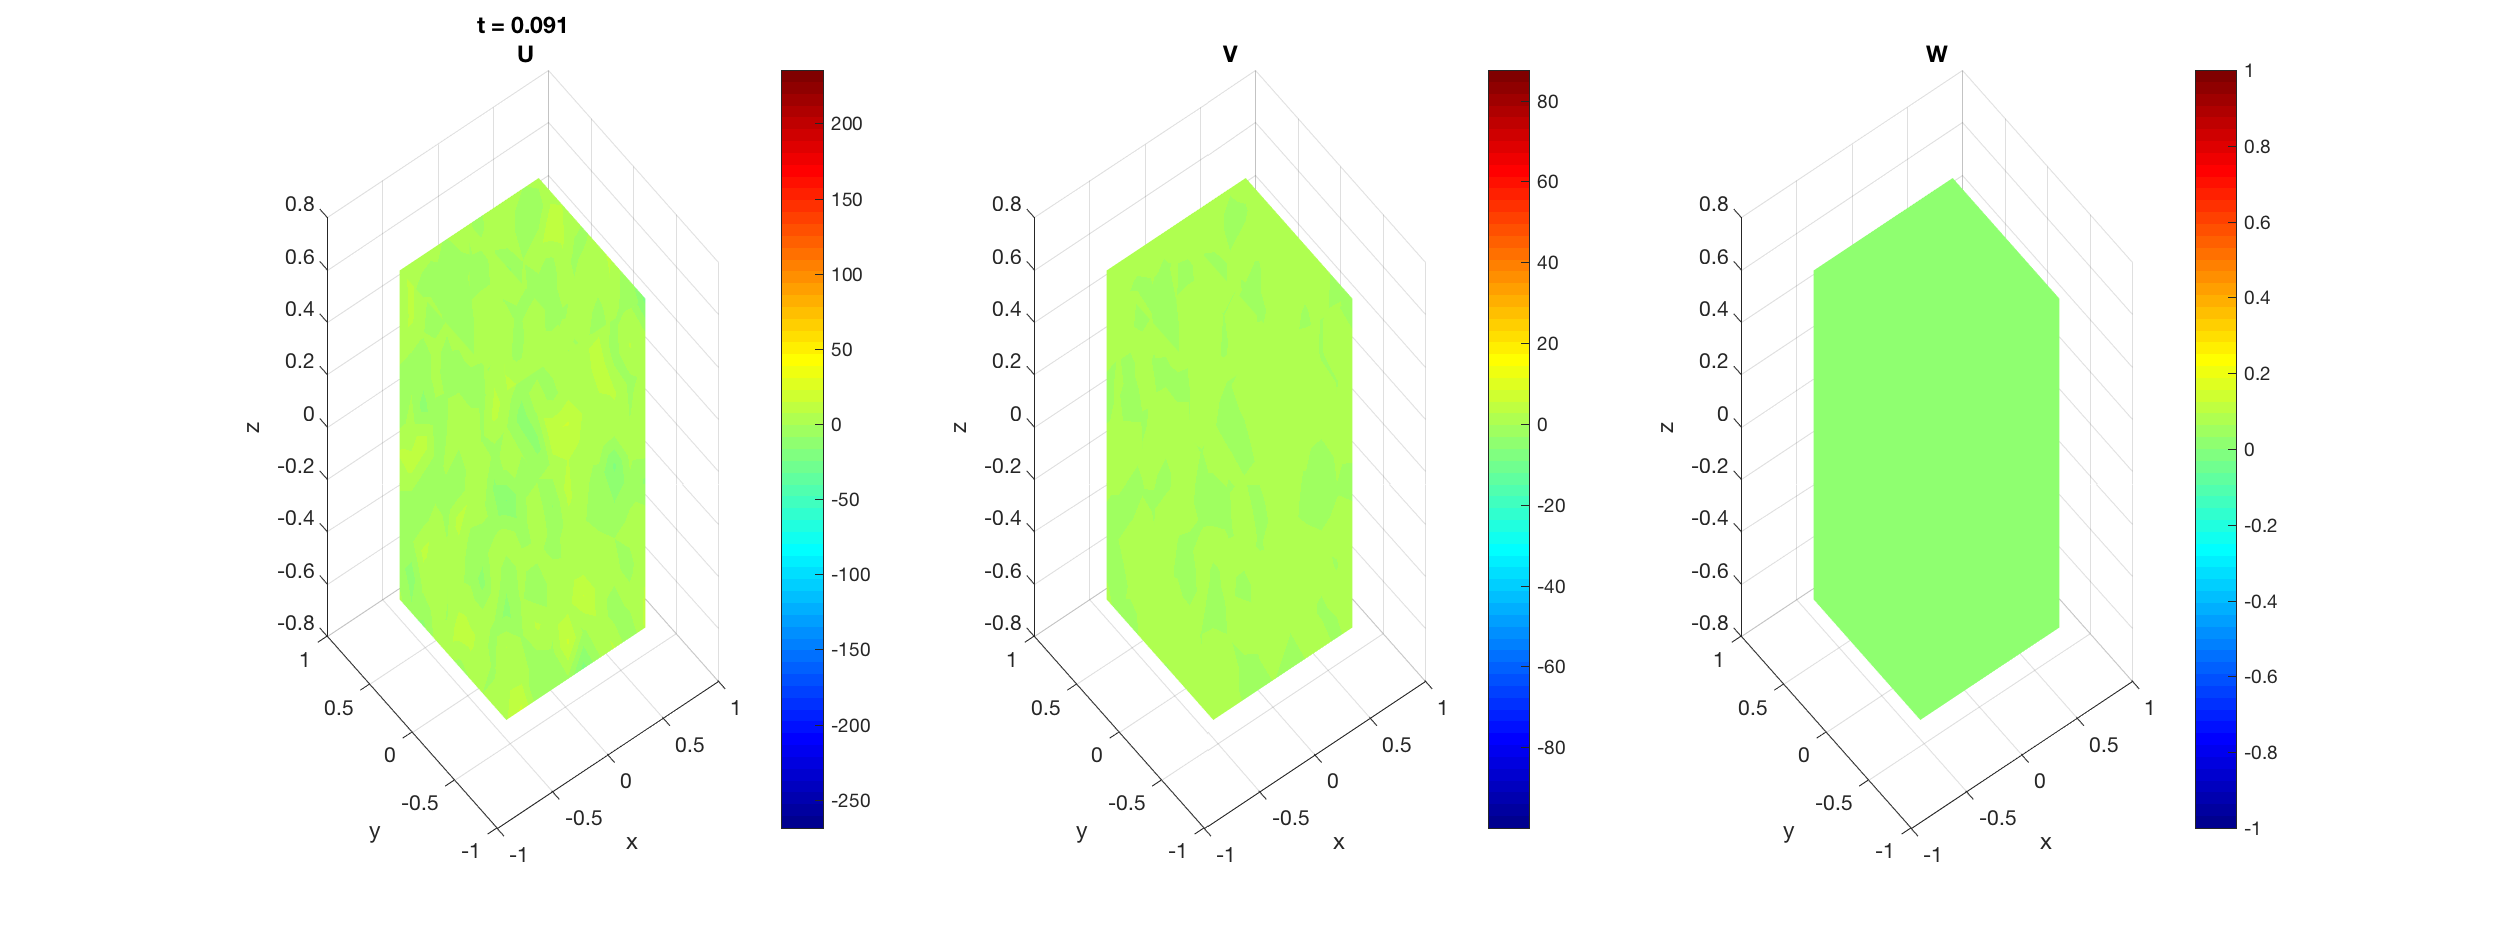
\includegraphics{../data/finalRuns/run2_frame10.png}}
        \caption{t = 0.091}
        \label{fig:frame2_10}
    \end{figure}
    \begin{figure}[H]
        \makebox[\textwidth]{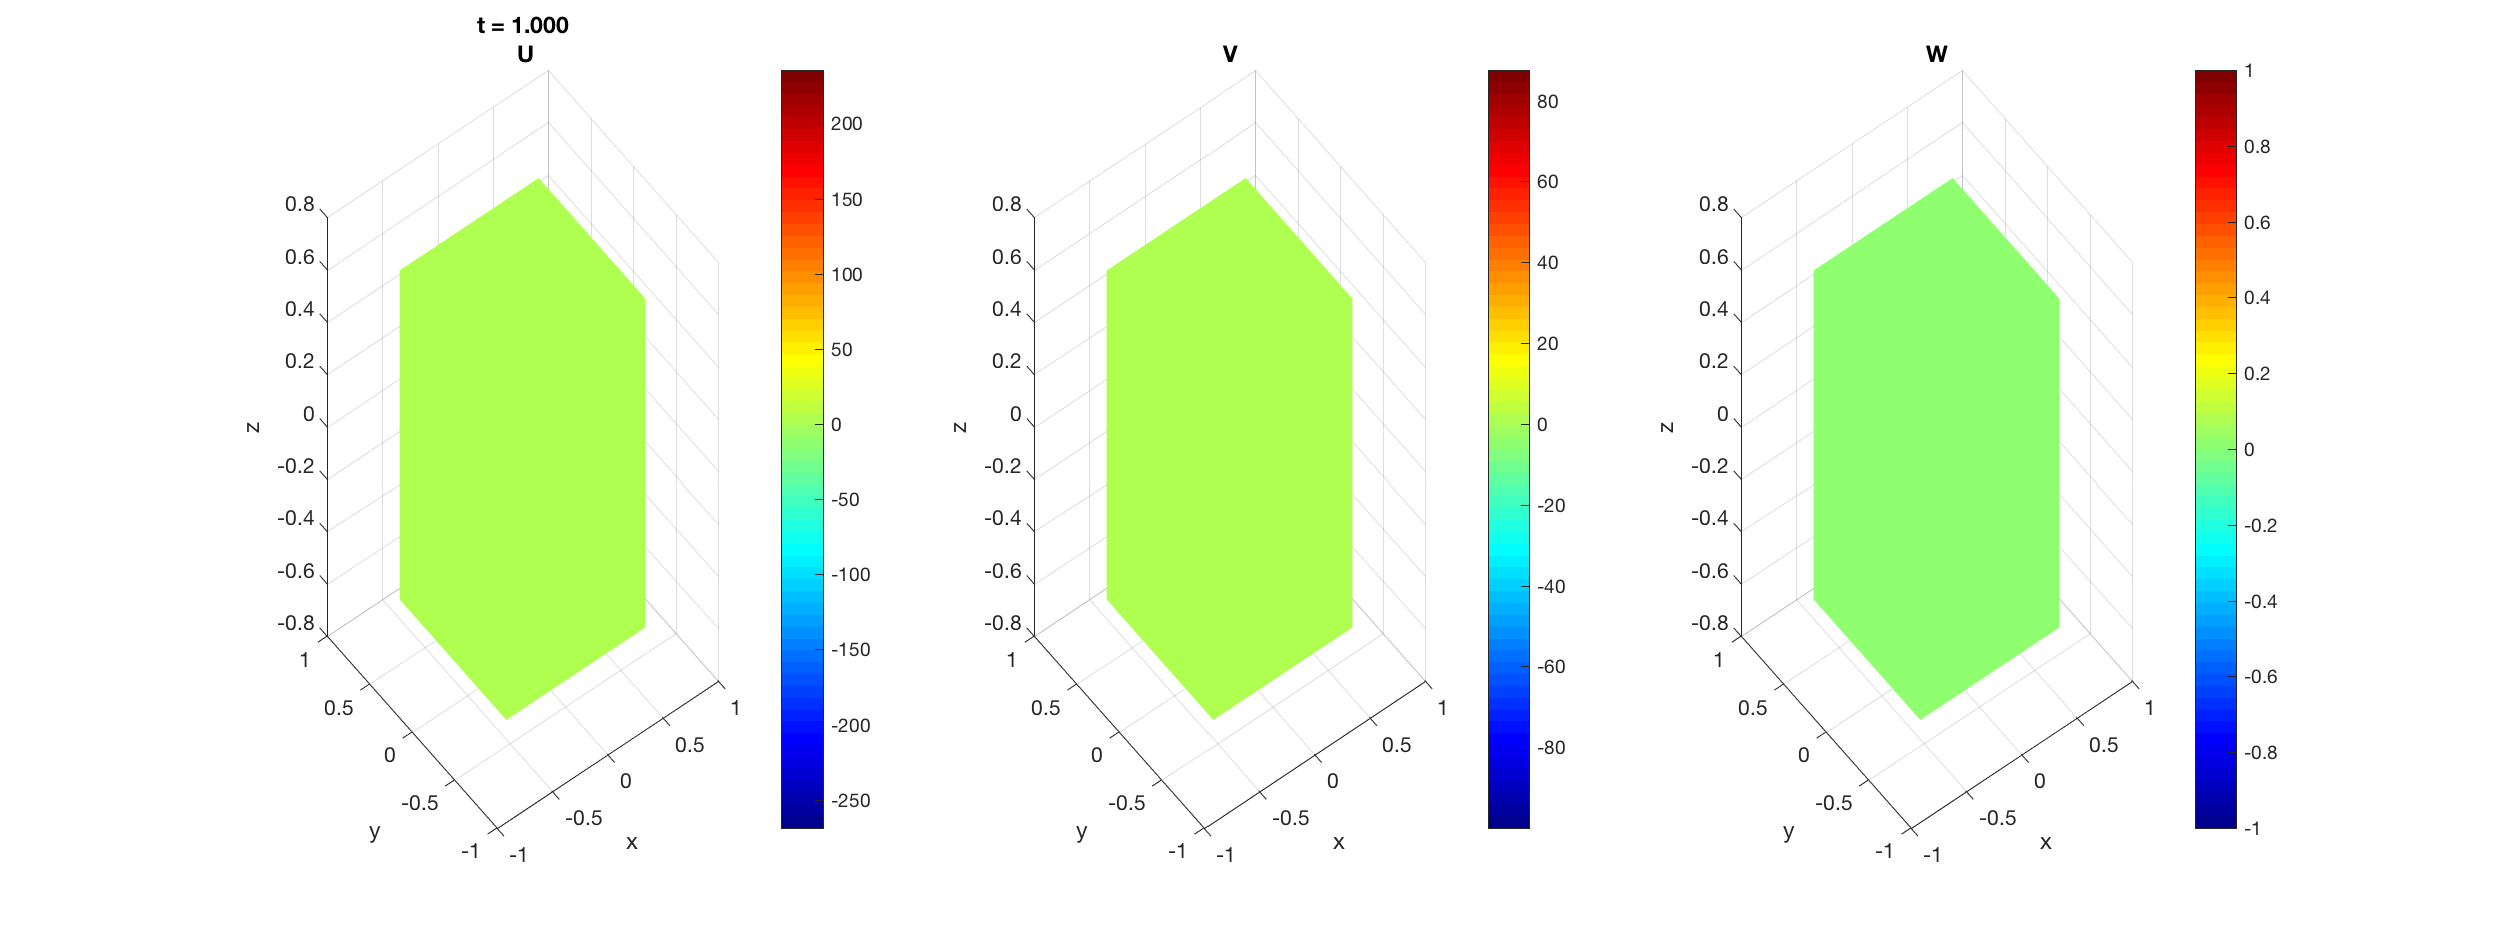
\includegraphics{../data/finalRuns/run2_frame100.png}}
        \caption{t = 1.0}
        \label{fig:frame2_100}
    \end{figure}


\subsubsection{Simulation 3: $\kappa$ as-is}
In this simulation, $\bm{\kappa} = [0.107, 0.144, 1.215 ]^T$.

    \begin{figure}[H]
        \centering
        \makebox[\textwidth]{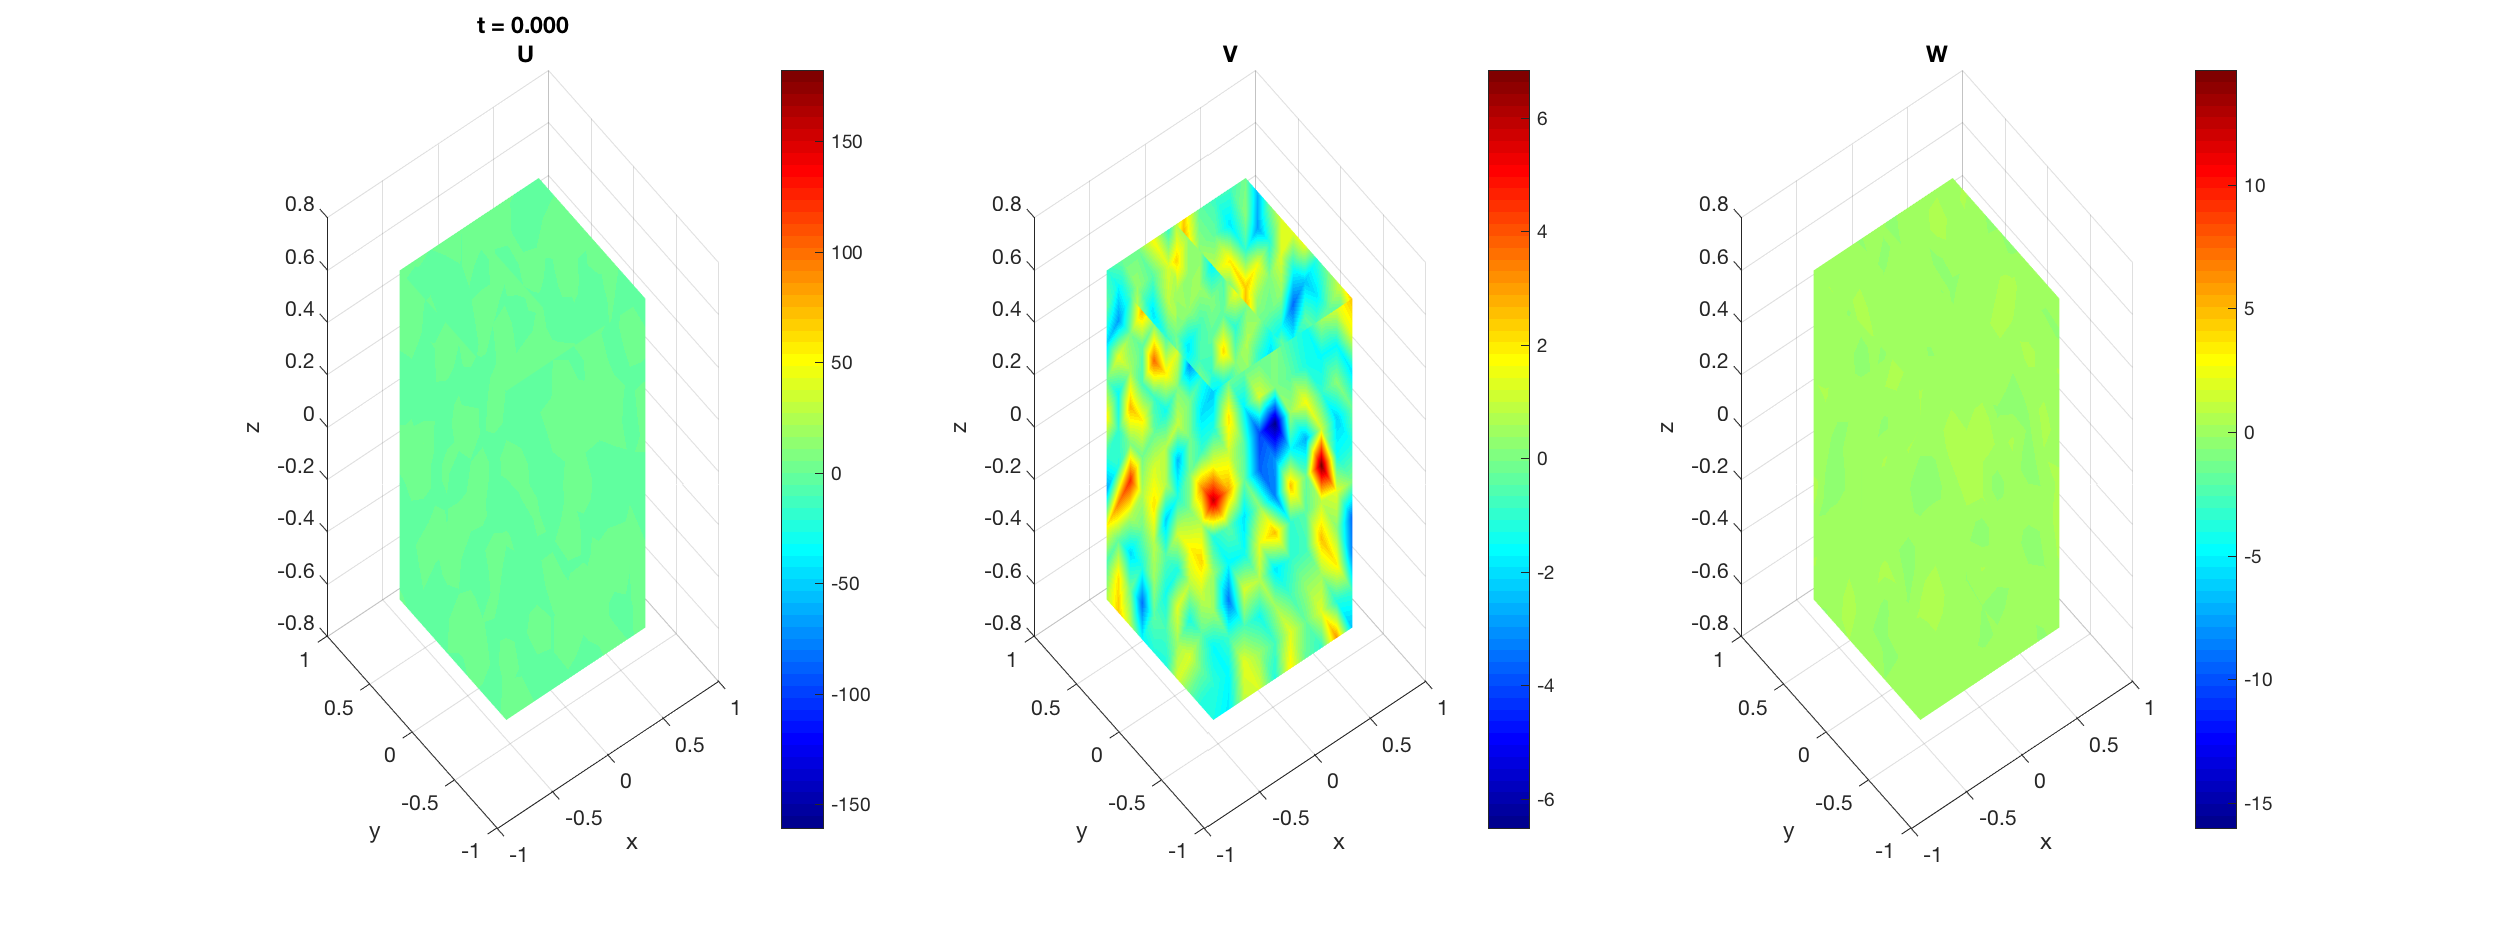
\includegraphics{../data/finalRuns/run3_frame1.png}}
        \caption{t = 0}
        \label{fig:frame3_1}
    \end{figure}
    \begin{figure}[H]
        \makebox[\textwidth]{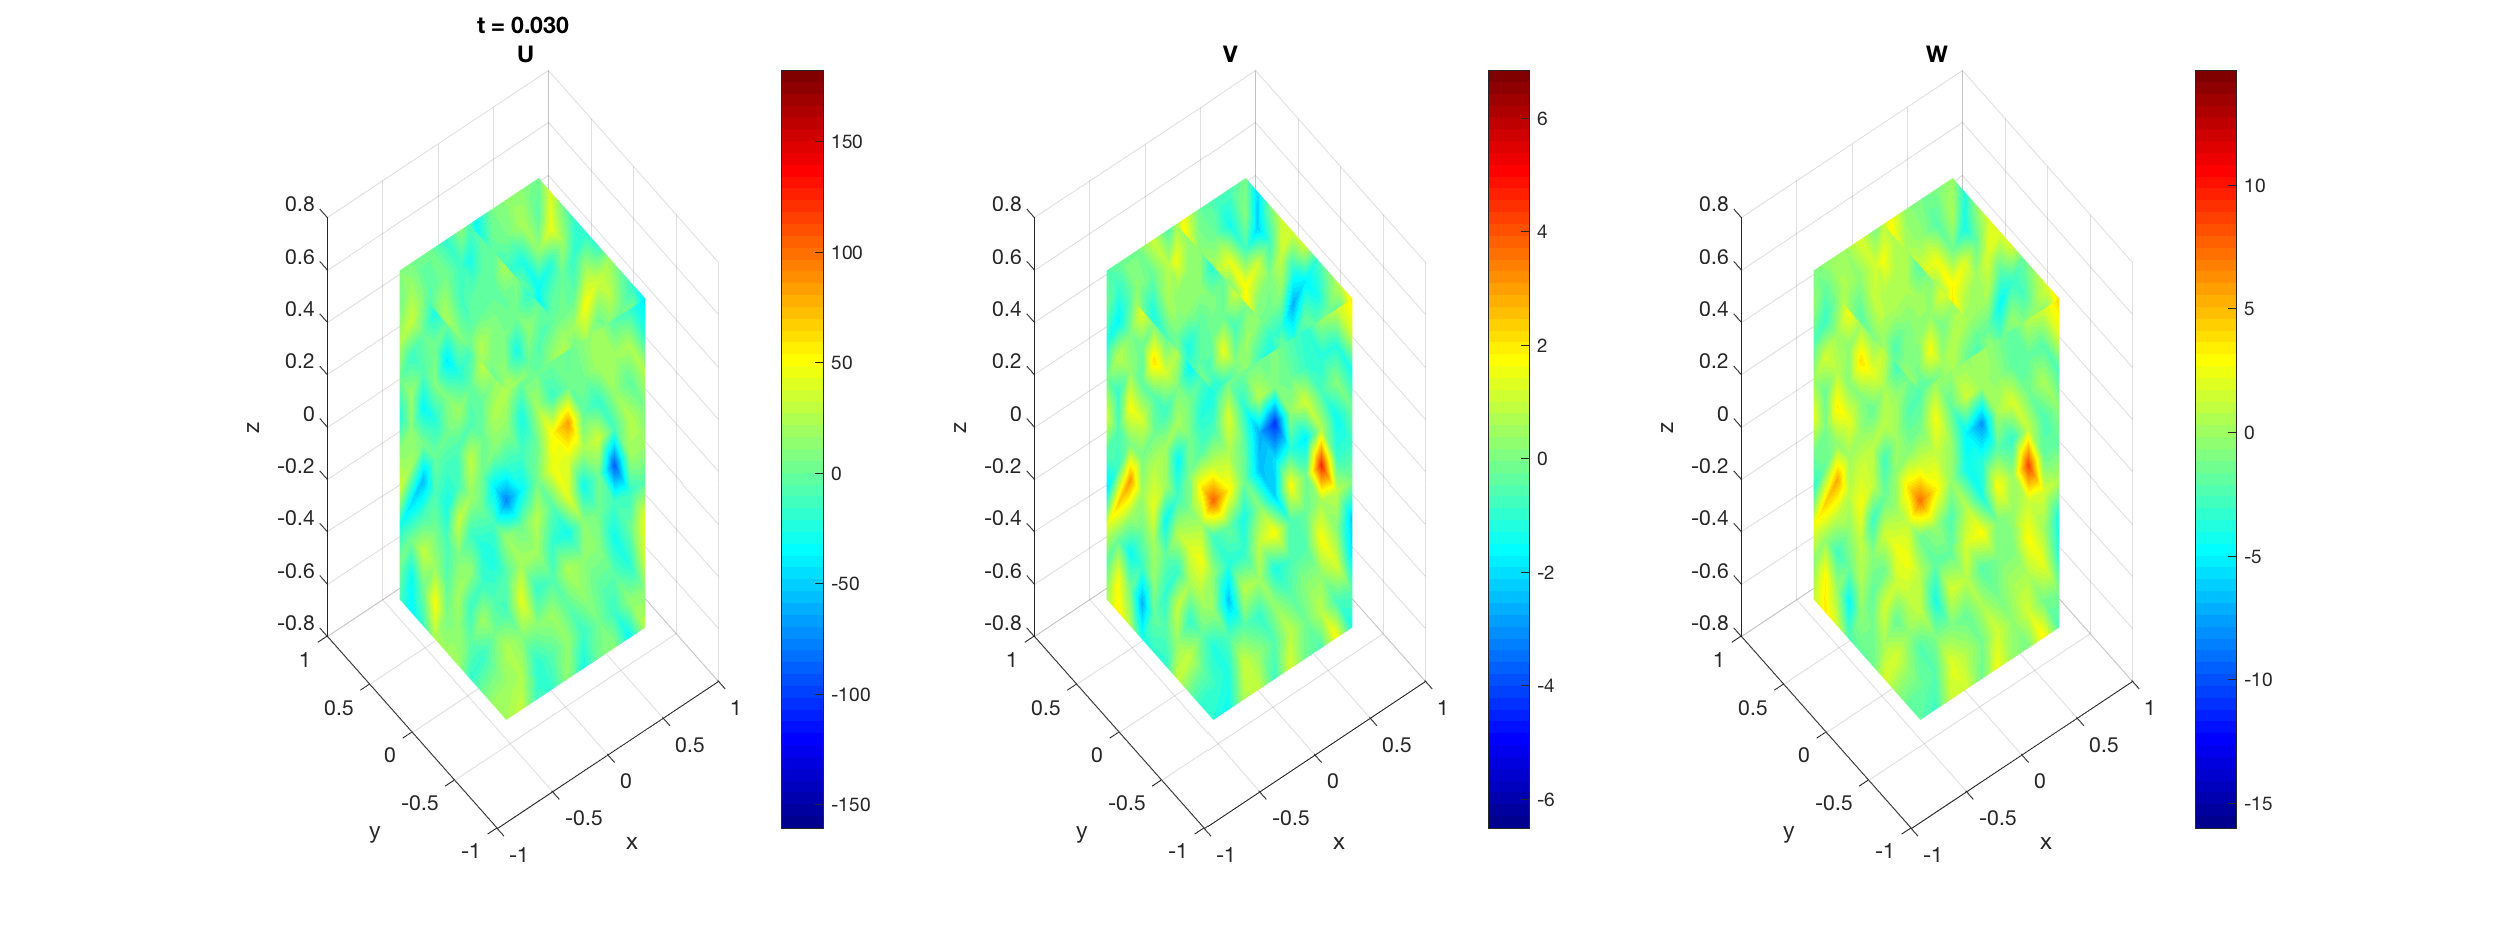
\includegraphics{../data/finalRuns/run3_frame4.png}}
        \caption{t = 0.030}
        \label{fig:frame3_4}
    \end{figure}
    \begin{figure}[H]
        \makebox[\textwidth]{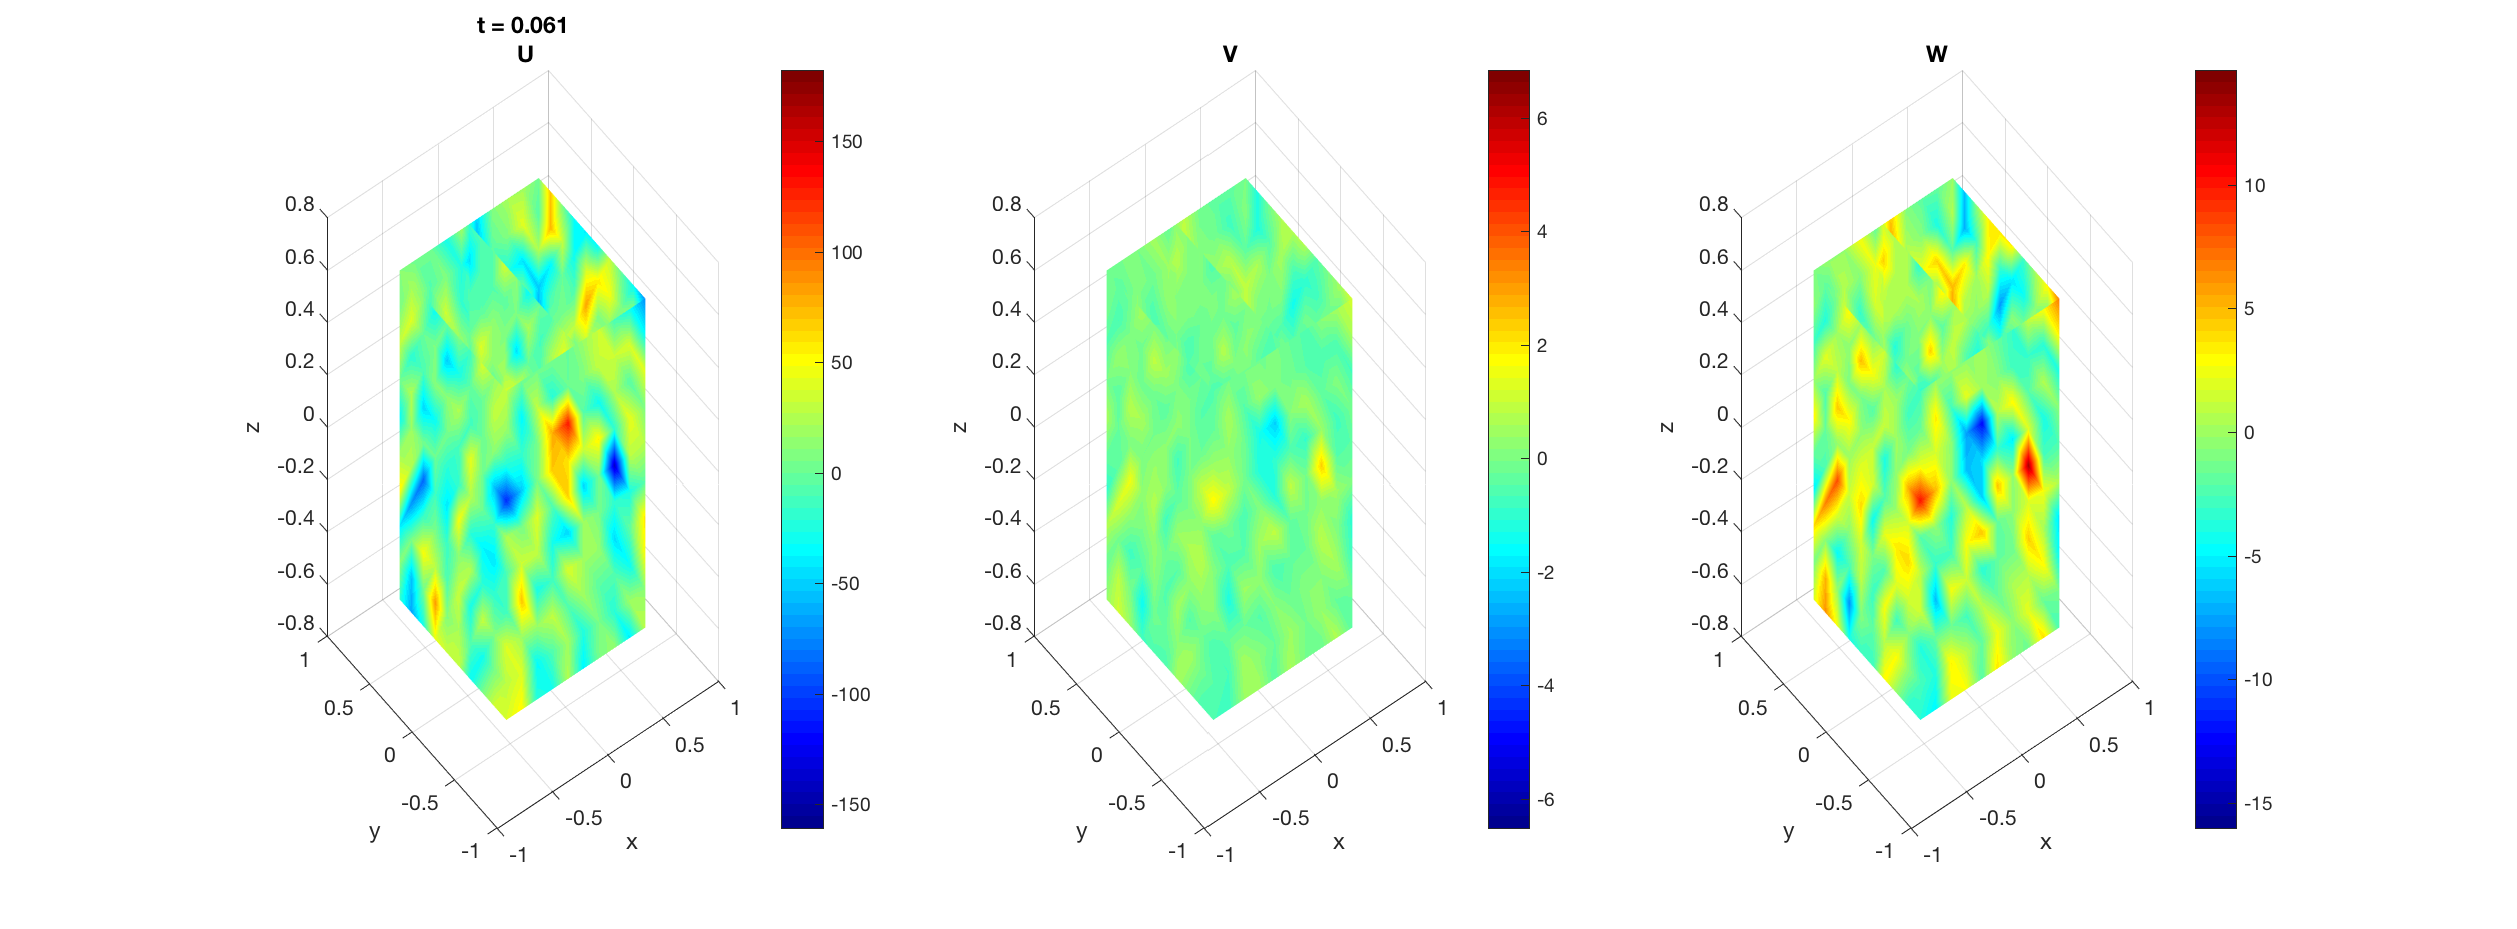
\includegraphics{../data/finalRuns/run3_frame7.png}}
        \caption{t = 0.061}
        \label{fig:frame3_7}
    \end{figure}
    \begin{figure}[H]
        \makebox[\textwidth]{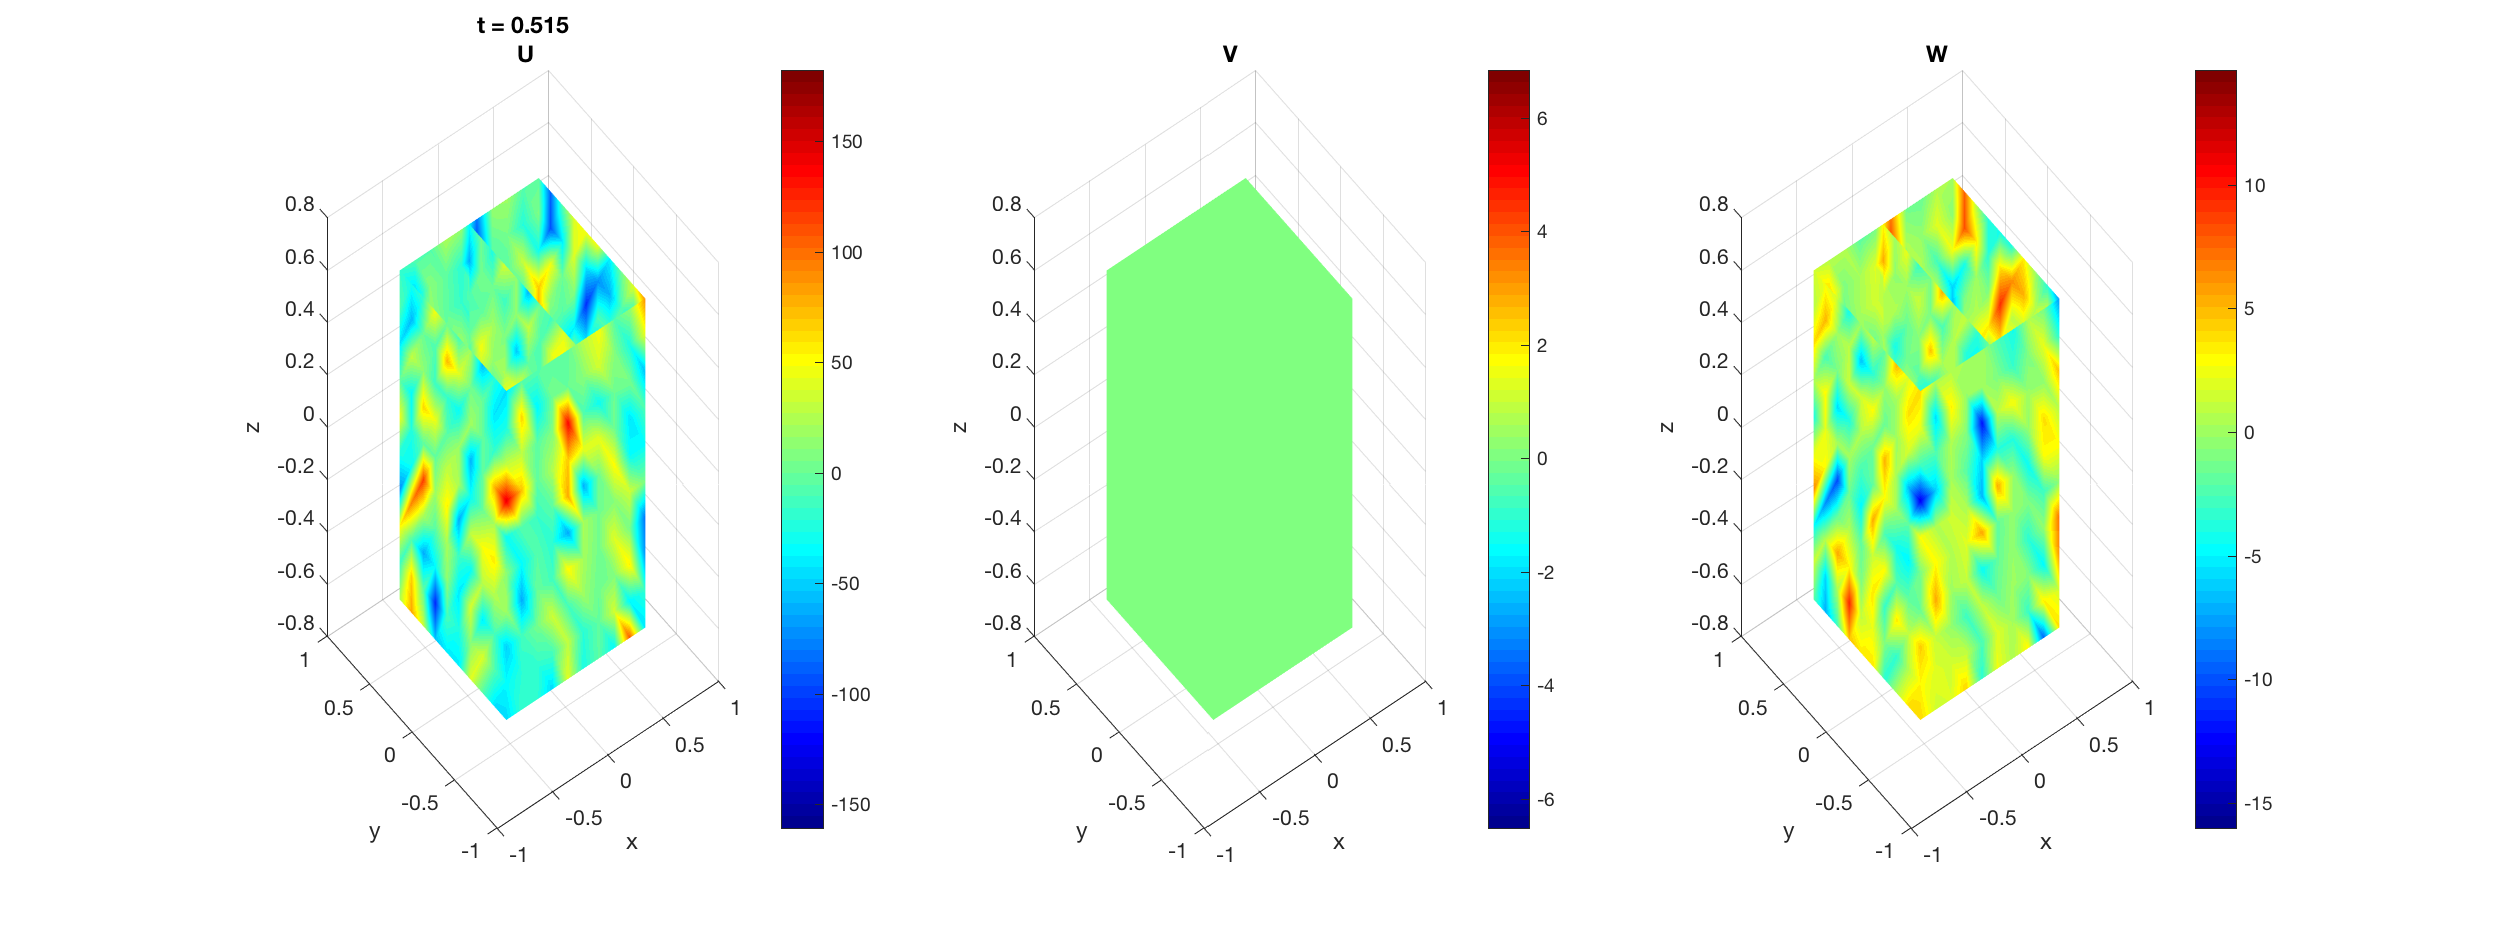
\includegraphics{../data/finalRuns/run3_frame52.png}}
        \caption{t = 0.515}
        \label{fig:frame3_67}
    \end{figure}
    \begin{figure}[H]
        \makebox[\textwidth]{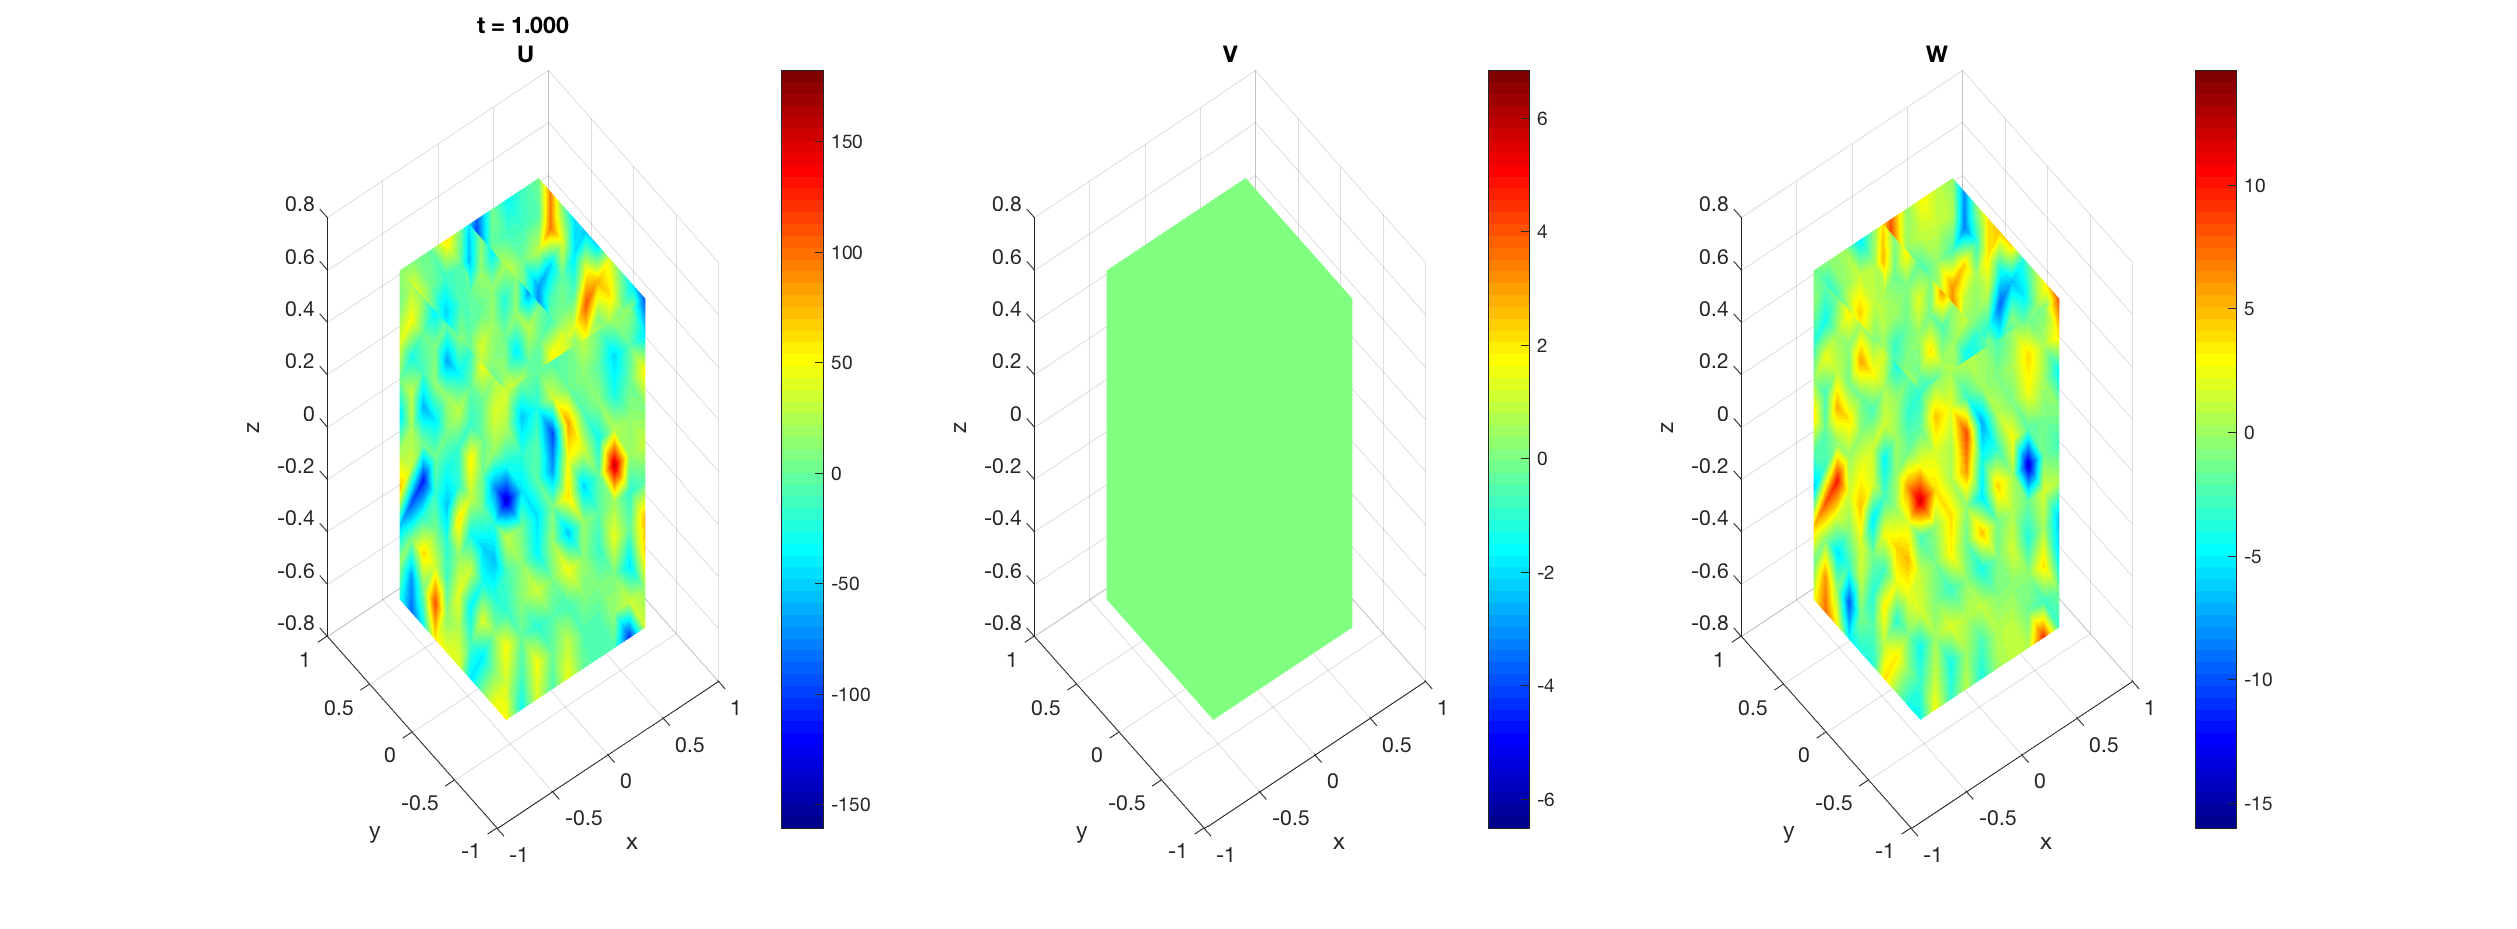
\includegraphics{../data/finalRuns/run3_frame100.png}}
        \caption{t = 1.0}
        \label{fig:frame3_100}
    \end{figure}



%----------------------------------------------------------------------------------------
%   PROBLEM 2
%----------------------------------------------------------------------------------------

\pagebreak
\section{Summary of Work}

\par
The first item action for beginning this independent study course involved studying the Navier-Stokes equations and the many definitions needed for an introduction to fluid mechanics and dynamics. This included becoming familiar with the notion of incompressibility, an intuitive sense of the difference between isotropic and anisotropic flow, and the differences between turbulent and non-turbulent flow. These basic concepts were not familiar to begin with, and it is essential to have a grasp of the underlying ideas before I can begin to apply these to numerical simulations. 

\par
After a few weeks of familiarizing myself with the background concepts -- and dealing with each authors' slightly different notation -- a \textsc{Matlab} function was written to visualize the three-dimensional fluid flow at a given time. For my style of learning, visualization is an important first step even if the initial conditions are unusable (for example, completely random instead of following the conditions for a zero-divergence flow field). The function for plotting the fluid field took about three hours total over a few days. Once this was in place, we could implement a basic numerical scheme (Fourth-Order Runge-Kutta) for solving the RDT differential equations. 

\par 
The RDT differential equations are defined in the Fourier space, and already spelled out clearly in the Pope text \cite{pope}. The assumptions we made to break the problem down even further was to use shear force. Dr. Lee derived these equations previously, and after following her notes, I was able to implement the equations.

\par
Numerically, roundoff error can cause an initially solenoidal field to develop non-zero divergence over time. In order to correct for buildup of error, we included a short "forcing function" to ensure that the field remained divergence-free for the duration of the simulation. A considerable amount of time was spent (and currently is being spent) here since zero-divergence in physical space is different than in Fourier space. Converting between the two can cause some errors that we are working on.

\par
The most challenging part of this course was getting a sense of the conversion between physical space and Fourier space. Theoretically, I understand the difference, but to identify the different moving parts for how the difference perspectives related to Rapid Distortion Theory was and still is a challenge. 

\par 
With the encouragement of Dr. Lee, we applied for a poster session at the American Physical Society Conference in March 2018. I would like to thank Dr. Lee for her responsiveness, continuous encouragement, and insight in keeping this project grounded and directed. 


%----------------------------------------------------------------------------------------
\pagebreak
\begin{thebibliography}{9}
\bibitem{pope}
Pope, Stephen B. \textit{Turbulent Flows}. Cambridge, Cambridge University Press, 2000.

\bibitem{reynoldsnumber}
Sommerfeld, Arnold (1908). "Ein Beitrag zur hydrodynamischen Erkläerung der turbulenten Flüssigkeitsbewegüngen (A Contribution to Hydrodynamic Explanation of Turbulent Fluid Motions)". \textit{International Congress of Mathematicians}. 

\bibitem{reynoldshistory}
Rott, N. (1990). "Note on the history of the Reynolds number". \textit{Annual Review of Fluid Mechanics}. 22 (1): 1–11.

\bibitem{potter} 
Potter, Merle C., and Wiggert, David C.
\textit{Mechanics of Fluids, 3rd Ed}. 
Brooks/Cole, California, 2002.

\bibitem{pedlosky}
Pedlosky, Joseph (1987). \textit{Geophysical fluid dynamics}. Springer. pp. 10–13. ISBN 978-0-387-96387-7.

\bibitem{nasa}
John V. Shebalin and Stephen L. Woodruff.
\textit{Kolmogorov flow in three dimensions}.
Physics of Fluids 1997 9:1, 164-170 

\end{thebibliography}

\end{document}